\documentclass[12pt]{article} 
\usepackage[utf8]{inputenc}
\usepackage{geometry}
\geometry{letterpaper}
\usepackage{graphicx} 
\usepackage{parskip}
\usepackage{booktabs}
\usepackage{array} 
\usepackage{paralist} 
\usepackage{verbatim}
\usepackage{subfig}
\usepackage{fancyhdr}
\usepackage{sectsty}

\setcounter{secnumdepth}{0}

\pagestyle{fancy}
\renewcommand{\headrulewidth}{0pt} 
\lhead{}\chead{}\rhead{}
\lfoot{}\cfoot{\thepage}\rfoot{}


%%% ToC (table of contents) APPEARANCE
\usepackage[nottoc,notlof,notlot]{tocbibind} 
\usepackage[titles,subfigure]{tocloft}
\renewcommand{\cftsecfont}{\rmfamily\mdseries\upshape}
\renewcommand{\cftsecpagefont}{\rmfamily\mdseries\upshape} %

\usepackage{amsmath}
\usepackage{amssymb}
\usepackage{bbm}
\usepackage{empheq}
\usepackage{xcolor}
\usepackage{tikz}
\usepackage{pgfplots}
\usepackage{listings}
\lstset{
  basicstyle=\ttfamily,
  mathescape
}

\pgfplotsset{width=10cm,compat=1.9}

\renewcommand{\L}[1]{\mathcal{L}\{#1\}}
\newcommand{\ans}[1]{\boxed{\text{#1}}}
\newcommand{\vecs}[1]{\langle #1\rangle}
\renewcommand{\hat}[1]{\widehat{#1}}
\newcommand{\F}[1]{\mathcal{F}(#1)}
\renewcommand{\P}{\mathbb{P}}
\newcommand{\R}{\mathbb{R}}
\newcommand{\qed}{\quad \blacksquare}
\newcommand{\brak}[1]{\langle #1 \rangle}
\newcommand{\E}{\mathbb{E}}
\newcommand{\bbm}[1]{\mathbbm{#1}}
\newcommand{\ind}{\mathbbm{1}}
\newcommand{\ellipsis}{\; \dots, \;}
\newcommand{\Var}{\text{Var}\;}
\newcommand{\mfX}{\mathfrak{X}}
\newcommand{\Z}{\mathbb{Z}}
\newcommand{\abs}[1]{\left\vert #1 \right\vert}
\newcommand{\mcC}{\mathcal{C}}
\newcommand{\iid}{\overset{iid}{\sim}}

\title{APMA 1690: Computational Probability and Statistics}
\author{Milan Capoor}
\date{Fall 2023}

\begin{document}
\maketitle
\tableofcontents

\textbf{Goal of the course:} (Approximately) Compute integrals using Monte Carlo methods

\section{Lecture 1: Sept 9}
\subsection{Arc of the Course}
\textbf{Example:} Motivating the goal of the course
\begin{align*}
    I &= \int_0^1 \arccos \left(\frac{\cos(\frac{\pi x}{2})}{1 + 2\cos(\frac{\pi x}{2})}\right)\; dx = \frac{5\pi}{12}
\end{align*}
This is \emph{really} hard! But using Monte Carlo methods we can do much better!

\textbf{Law of Large Numbers:} Suppose $X_1, \, ...., X_n$ are independently and identically distributed random variables. Then, when $n \to +\infty$,
\[\frac{1}{n}\sum_{i=1}^n f(X_i) \to \E [f(X_1)]\]

If we define $X_1 \sim \text{Unif}(0, 1)$, then the PDF of $X_1$ is 1. 

Applying this to the integral above, let the integrand be denoted $f(x)$ so 
\[I = \int_0^1 f(x)\; dx = \int_0^1 f(x) \cdot 1 \; dx = \E [f(X_1)]\]

Putting all of this together, 
\[I = \E[f(X_1)] \approx \frac{1}{n} \sum_{i=1}^n f(X_i)\]
which means that by doing some transformations on the integral and averaging many random outputs of the integrand, we can use the average to approximate the value of the integral with good accuracy. 

In fact, with $n=10000$, we approximate $I = 1.308827$ when in fact $I = \frac{5\pi}{12} \approx = 1.308997$ which is quite good!

\textbf{A problem:} Notice! This method \emph{assumes} we are able to generate iid random variables. This introduces some questions:
\begin{enumerate}
    \item What is ``randomness''?
    \item How do we generate random numbers?
    \item How large is our error when using stochastic methods? How do we control this error?
    \item What if the inputs are random vectors instead of random numbers? What if the problem is multi-variable?
    \item How do we manage unreasonable time and memory costs?
\end{enumerate}

\textbf{Moving towards a solution:} To address the last concern especially, we can compromise on the iid condition to generate a Markov chain where $\vec{X}_n \dot \sim \Pi$

\textbf{Heuristic Ergodic Theorem:}
Suppose $\vec{X}_1, \vec{X}_2,\, ..., \vec{X}_n$ is a Markov chain such that $\vec{X}_n \dot \sim \Pi$ when n is large. Then 
\[\frac{1}{n} \sum_{i=1}^n f(\vec{X}_i) \approx \int f(x) \cdot \Pi(x)\; dx\]

Really, this just introduces more questions:
\begin{enumerate}
    \setcounter{enumi}{5}
    \item What is the ergodic theorem?
    \item How do we generate a Markov chain satisfying this assumption that $\vec{X}_n \dot \sim \Pi$?
\end{enumerate}

This will lead us to two algorithms:
\begin{itemize}
    \item Metropolis-Hastings Algorithm
    \item Gibbs sampling (developed by Prof Geman at Brown!)
\end{itemize}

\subsection{Random Variables}
\textbf{Example: Coin toss}

With a sample space $\Omega = \{H, T\}$, let $X$ represent the outcome of flipping the coin once. Then really, $X : \Omega \mapsto \{0, 1\}$.

In fact, this gives us a formal definition for a \emph{random variable}; a random variable is a function $X$ that maps a sample space $\Omega$ to $\R$.
\[\text{For each fixed } \omega \in \Omega, \quad X(\omega) \in \R\]

\section{Lecture 2: Sept 12}
\textbf{What is randomness?}

\subsection{Probability Theory}
\begin{enumerate}
    \item Sample Space ($\Omega$)
    \item Random Variable ($X$)
    \item Probability ($\P$)
\end{enumerate}

\textbf{Sample space:} the collection of all possible outcomes of an event 
\emph{Examples:}
\begin{itemize}
    \item For flipping a coin once, $\Omega = \{H, T\}$
    \item Rolling a six sided die, $\Omega = \{1, 2, 3, 4, 5, 6\}$
\end{itemize}

\textbf{Remark:} the essential characteristic of experiments in sample space is that the outcome in uncertain before performing the experiment.

\textbf{Event:} $A \subseteq \Omega$

\textbf{Random Variable:} a function $X: \Omega \to \R^d$ 

\textbf{Deterministic/Pseudo-Random Variable:} $x \in \R^d, \quad X(\omega) = x, \; \forall \omega \in \Omega$

\textbf{Probability:} a real-valued function of all subsets of omega ($\P: A \to \R \quad A \subseteq \Omega)$ which satisfies the following three axioms:
\begin{enumerate}
    \item $\forall A \subseteq \Omega, \quad \P(A) \geq 0$
    \item $\P(\Omega) = 1$
    \item $\forall \{A_n\}_{n=1}^\infty \subseteq \Omega \text{ such that } A_i \cap A_j = \emptyset \; (i \neq j)$ (for any mutually exclusive infinite sequence of events),
    \[\P\left(\bigcup_{n=1}^\infty A_n\right) = \sum_{n=1}^\infty \P(A_n)\]
\end{enumerate}

\textbf{Theorem:} The probability of an impossible event is 0.

\emph{Proof:} 
Let $A_n = \emptyset \quad n = \{1, 2, \,..., n\}$. Clearly, for any $i \neq j$, 
\[A_i \cap A_j = \emptyset \cap \emptyset = \emptyset\] 
so 
\begin{align*}
    \P\left(\bigcup_{n=1}^\infty A_n\right) &= \sum_{n=1}^\infty \P(A_n)\\
    \P\left(\bigcup_{n=1}^\infty \emptyset\right) = \P(\emptyset) &= \sum_{n=1}^\infty \P(\emptyset)
\end{align*}
Define $a := \P(\emptyset)$. Then, 
\[a = \sum_{n=1}^\infty a\]
so $a = 0 \implies \P(\emptyset) = 0 \qed$

\section{Lecture 3: Sept 14}
\subsection{Indicator Functions}
\textbf{Definition:} Let $A \subseteq \R^d$, 
\[\mathbbm{1}_A(x) = \begin{cases}
    1 \quad x \in A\\
    0 \quad x \not \in A
\end{cases}\]

\textbf{Examples:}
\begin{enumerate}
    \item $d=1, \quad A = (0, 1) \subseteq \R^1$
    \[\bbm{1}_{(0, 1)}(x) = \begin{cases}
        0 \quad x \leq 0\\
        1 \quad 0 < x < 1\\
        0 \quad x \geq 1
    \end{cases} \]

    \item $d = 1, \quad A = [0, +\infty)$ (Heaviside function)
    \[\bbm{1}_{[0, \infty)} = \bbm{1}(x \geq 0) = \begin{cases}
        1 \quad x \geq 0 \\
        0 \quad \text{otherwise}
    \end{cases}\]
\end{enumerate}

\subsection{Interlude: Probability theory vs. Statistics}
Probability seeks to establish the expected outcome of an experiment before it is performed, given $\P$.

Statistics seeks to infer $\P$ from data observed during the experiment. 

\subsection{Distribution}
\textbf{Definition:} Let $X$ be a $\R^d$-valued RV defined on the probability space $(\Omega, \P)$. Then, the distribution of $X$ according to $\P$ is 
\[\P\left(\left\{ \omega \in \Omega: X(\omega) \in A \right\}\right) \quad \forall A \subseteq \R^d\]

\textbf{Remarks:}
\begin{itemize}
    \item To study the distribution of $X$ we must examine all $A \subseteq \R^d$ which is very hard 
    \item When $d=1$ this is easier because we must only examine the interval of the form $(-\infty, t] \quad \forall t\in \R$
\end{itemize}

\subsection{Cumulative Distribution Functions (CDFs)}
\textbf{Definition:} Let $X: (\Omega, \P) \to \R$. Then the CDF of $X$ is $F_X: \R \to \R$
\[F_X(t) := \P\left(\{\omega \in \Omega : X(\omega) \leq t\}\right)\]

\textbf{Examples:}
\begin{itemize}
    \item $X \sim \text{Exp}(\lambda)$
    \[F_X(t) = (1 - e^{-\lambda t}) \cdot \bbm{1}(t \geq 0 )\]
    \begin{center}
        \begin{tikzpicture}
            \begin{axis}[
                yticklabels={0, , , , , , 1}, 
                xticklabels={,},
                axis lines=left, 
                xlabel=$t$, 
                ylabel=$F_X$
            ]
                \addplot[blue, domain=0:10, label=($F_X$)]{1 - e^(-x)};
                \addplot[red, dashed, domain=0:10, label=1]{1};
            \end{axis}
        \end{tikzpicture}
    \end{center}

    \item $X \sim \text{Bernoulli}(\frac{1}{2})$
    \[F_X(t) = \begin{cases}
        0 \quad t <0\\
        \frac{1}{2} \quad 0 \leq t< 1\\
        1 \quad t \geq 1
    \end{cases}\]
    
    \begin{center}
        \begin{tikzpicture}
            \begin{axis}[
                xticklabels={, $0$, , , $1$},
                ytick={0, 0.25, 0.5, 0.75, 1}, 
                yticklabels={$0$, ,$\frac{1}{2}$, , $1$},
                axis lines=middle
            ]
                \addplot[blue, very thick, domain=-1:0,]{0};
                \addplot[blue, very thick, domain=0:1]{0.5};
                \addplot[blue, very thick, domain=1:2]{1};
            \end{axis}
        \end{tikzpicture}
    \end{center}
\end{itemize}

\subsection{Continuous Random Variables}
\textbf{Definition:} Let $X : (\Omega, \P) \to \R$. If its CDF is continuous and piecewise differentiable (``absolutely continuous'') then $X$ is a \emph{continuous random variable}

\textbf{Probability Density Function (PDF):} 
\[p_X(t) := \frac{d}{dt}F_X(t)\]
where $\frac{d}{dt}$ is the piecewise derivative. 

\textbf{Remarks:} the CDF determines the corresponding PDF via differentiation and the PDF determines the CDF via integration
\begin{align*}
    p_X(x) &= \frac{d}{dx} F_X(x)\\
    F_X(x) &= \int_{-\infty}^t p_X(t)\; dt
\end{align*}

\textbf{Theorem:} Let $X : (\Omega, \P) \to \R$. 
\begin{enumerate}
    \item $F_X(t)$ is non-decreasing: $F_X(t_1) \leq F_X(t_2)$ if $t_1 \leq t_2$
    \item $\lim_{t\to -\infty} F_X(t) = 0, \quad \lim_{t\to \infty} F_X(t) = 1$ 
\end{enumerate}

\section{Lecture 4: Sept 19}
\subsection{CDFs}
The CDF of $X \sim \text{Bernoulli}(\frac{1}{3})$ can be written in a number of ways.

First, by probabilities, 
\[\begin{cases}
    \P(X = 1) = \frac{1}{3}\\
    \P(X = 0) = \frac{2}{3}
\end{cases}\]

Which yields a CDF
\[F_X(t) = \begin{cases}
    0 \quad t < 0\\
    \frac{2}{3} \quad 0 \leq t < 1\\
    1 \quad t \geq 1
\end{cases}\]

Which describes
\[F_X(t) = \frac{2}{3} \ind_{(t \geq 0)}(t) + \frac{1}{3}\ind_{(t \geq 1)}(t) = \sum_{k=0}^1 p_k \cdot \ind_{(t\geq x_k)}(t)\]
where $x_0 = \P(X = 0)$ and $x_1 = \P(X = 1)$

\subsection{Discrete Random Variables}
\textbf{Definition:} Let $X$ be $\R^1$-valued RV on $(\P, \Omega)$. $X$ is a discrete RV if its CDF is
\[F_X(t) = \sum_{k=0}^K p_k \cdot \ind_{(t \geq x_k)}(t)\]
where $\{x_k\}_{k=0}^K$ are distinct real numbers, $\{p_k\}_{k=0}^K$ are non-negative real numbers satisfying $\sum_{k=0}^K p_k = 1$ and $K$ is a positive integer (or $+\infty$)

\textbf{Probability Mass Function (PMF):} the ordered sequence $\{p_k\}_{k=0}^K$ which determines the CDF. 

\textbf{Theorem (Non-rigorously):} For a discrete RV, 
\[p_k = \P(X = k)\]

\subsection{Mixed Random Variables (Optional)}
\textbf{Example:} Let $Y \sim \text{Bernoulli}(\frac{1}{2})$ and $Z\sim N(0,1)$ be independent RVs on $(\Omega, \P)$. 
\[X(\omega) := Y(\omega) + (1 - Y(\omega)) \cdot Z(\omega)\]

Note that $X$ is a RV because $X : \Omega \to \R$. 

\subsection{Expected Values}
\textbf{Notation:} Let $g: \R \to \R$ and $X: \Omega \to \R$. Then $g(X(\omega)) : \Omega \to \R$ so we denote $g(X)$ as a random variable. 

\textbf{Definition:}
Let $g : \R \to \R$. 

\begin{enumerate}
    \item Suppose $X$ is a continuous RV whose PDF is $p_X$.
    
    If $\int_{-\infty}^{\infty} |g(x)| \cdot p_X(x)\; dx < \infty$, 
    \[\E[g(X)] := \int_{-\infty}^{\infty} g(x)\cdot p_X(x)\; dx\]
    otherwise, $\E[g(X)]$ does not exist.

    \item Suppose $X$ is a discrete RV with CDF $F_X(t) = \sum_{k=0}^k p_k \cdot \ind_{(t\geq x_t)}(t)$. 
    
    If $\sum_{k=0}^K |g(x_k)| \cdot p_k < \infty$, then 
    \[\E[g(X)] := \sum_{k=0}^K g(x_k) \cdot p_k\]
    otherwise, $\E[g(X)]$ does not exist.
\end{enumerate}

\section{Lecture 5: Sept 21}
\subsection{Law of Large Numbers (LLN)}
\textbf{Theorem:} Let $X_1,\; \dots, \; X_n$ be $\R^1$-dimensional RVs on $(\Omega, \P)$. If the RVs are independently and identically distributed and $\E[X_1]$ exists, then 
\[\boxed{\P\left(\left\{\omega \in \Omega: \lim_{n\to\infty} \left(\frac{1}{n}\sum_{i=1}^n X_i(\omega)\right) = \E X_1\right\}\right) = 1}\]

\textbf{Corollary:} Under the same conditions, 
    \[\P\left(\left\{\omega \in \Omega: \lim_{n\to \infty} \left(\frac{1}{n}\sum_{i=1}^n X_i(\omega)\right) \neq \E X_1\right\}\right) = 0\]

\textbf{Remarks:}
\[\overline X_n(\omega) := \frac{1}{n}\sum_{i=1}^n X_i(\omega)\]
Then the following are all random variables:
\begin{itemize}
    \item $\overline X_n$
    \item $\lim_{n\to\infty} \overline X_n(\omega)$
    \item $e_n(\omega) := |\overline X_n(\omega) - \E X_1|$
\end{itemize}

So the LLN can also be written as 
\[\P(\{\omega \in \Omega: \lim_{n\to\infty} e_n(\omega) = 0\}) = 1\]

\subsection{Law of the Iterated Logarithm}
\textbf{Variance:}
\[\Var(X) = \E(X^2) - (\E X)^2\]

\textbf{Theorem:} Let $X_1, X_2, X_3,...$ be identically and independently distributed RVs defined on $(\Omega, \P)$ Suppose $\E X_1$ and $\text{Var}(X_1)$ exist. 
Then, 
\[\P\left(\{\omega \in \Omega : \lim_{m \to \infty} \left[
\sup_{n \geq m} \left(\frac{e_n(\omega)}{\sqrt{\text{Var}X_i \frac{2\log(\log n)}{n}}}\right)\right] = 1\}\right) = 1\]

Heuristically, when n is large,
\begin{empheq}[box=\fbox]{align*}
    \P(\{\omega \in \Omega : |e_n(\omega)| \leq \sqrt{\text{Var}X_i \frac{2\log(\log(n))}{n}}\}) &\approx 1\\
    \P(\{\omega \in \Omega : |e_n(\omega)| > \sqrt{\text{Var}X_i \frac{2\log(\log(n))}{n}}\}) &\approx 0\\
\end{empheq}

\subsection{Empirical CDFs}
\textbf{Definition:} Suppose $X_1, \ellipsis X_n$ are RVs defined on $(\Omega, \P)$. 
\[F_n(\omega, t) = \frac{1}{n}\sum_{i=1}^n \ind_{t \geq X_i(\omega)}(t)\]

For each fixed $\omega$, $F_n$ is a function of $t$. For each fixed $t$, $F_n$ is a random variable. Therefore, $F_n$ is a \emph{stochastic process}

If $X_1, \ellipsis X_n \overset{iid}{\sim} F$, we would like to use $F_n(\omega, t)$ to estimate $F$:
\[|F_n(\omega, t) - F(t)| \overset{?}{\approx} 0\]

\subsection{Glivenko-Contelli Theorem (1933)}
\textbf{Theorem:} Suppose $X_1, \ellipsis X_n$ are RVs defined on $(\Omega, \P)$. If the RVs are iid, then 
\[\P(\{\omega \in \Omega: \lim_{n\to \infty} \max_t|F_n(\omega, t) - F(t)| = 0\}) = 1\]

In other words, ``$F_n(\omega, t)$ converges to $F$ uniformly in $t$ with probability 1.''

\section{Lecture 6: Sept 26}
\subsection{True-Random Numbers}
\textbf{Definition:} Real numbers $x_2, x_2, \ellipsis x_n$ are called \emph{random numbers} from a distribution associated with a CDF if 
\begin{enumerate}
    \item there is an underlying probability space $(\Omega, \P)$
    \item $\exists X_1, X_2, \ellipsis X_n$ are iid random variables defined on $(\Omega, \P)$ which share the CDF $F$
    \item 
    \[\exists \omega^* \in \Omega: \begin{cases}
        x_1 = X_1(\omega^*)\\
        x_2 = X_2(\omega^*)\\
        \qquad \vdots\\
        x_n = X_n(\omega^*)
    \end{cases}\]
\end{enumerate}

\textbf{Remarks:}
\begin{enumerate}
    \item Each RV $X_i$ mainly refers to a truly random RV ($X_i$ is not a constant function)
    \item A random variable $X_i(\omega)$ is a function $\omega \to \R$
    \item A random number $x_i = X_i(\omega^*)$ is a number in $\R$
\end{enumerate}

\subsection{Types of Random Number Generators}
\begin{enumerate}
    \item Hardware RNGs
    \begin{itemize}
        \item \emph{Pros:} create true random numbers
        \item \emph{Cons:} slow and expensive
    \end{itemize}

    \item Pseudo RNGs
    \begin{itemize}
        \item \emph{Pros:} Very fast 
        \item \emph{Cons:} Not truly random
    \end{itemize}
\end{enumerate}

\subsection{Pseudo-random Number Generators}
\textbf{Definition:} Suppose $F$ is a given CDF. Let $g: \{1, 2, 3, \ellipsis\} \to \R$ be a function. $g$ is called a PRNG for $F$ if 
\[\lim_{n\to \infty} \left(\sup_t\bigg \vert \frac{1}{n}\sum_{i=1}^n \ind_{(t \geq g(i))} - F(t) \bigg \vert\right)\]
and the outputs of $g$ are pseudo-random numbers.

Essentially, \emph{the numbers $g(i)$ look like true-RNs iid from F but are not}.

\textbf{Glivenko-Contelli theorem vs PRNGs:}

The essence of the GCT is that the empirical CDF of a sequence of iid RVs converges to the true CDF. PRNGs, meanwhile, function in the reverse direction: when the empirical CDF converges to F, the random variables look like true iid RVs. 

\textbf{Example:} the Multiplicative Congruential Generator (MCG)

Let $X$ be a RV defined on $(\Omega, \P)$ and $m \in \mathbb{N}$. We say $X \sim \text{Unif}(\{1, 2, \ellipsis m-1\})$ so 
\[\P(X = i) =  \frac{1}{m - 1} \quad 1 \leq i \leq m-1\]
\[\implies F_X(t) = \frac{1}{m -1}\sum_{i=1}^n \ind_{(t \geq i)}\]

\emph{The Algorithm:}
\begin{itemize}
    \item Input: 
    \begin{enumerate}
        \item `properly chosen'' integers $m$ and $a$ (in an old version of Matlab, they used $m = 2^{31} - 1$ and $a = 7^5$) where ``properly chosen'' involves lots of number theory
        \item a seed $s$
        \item a sample size $n$
    \end{enumerate}

    \item Output: $g(1), g(2), \ellipsis g(n)$ which look like iid random numbers from $\text{Unif}(\{1, 2, \ellipsis m-1\})$
\end{itemize}

Process:
\begin{verbatim}
    g(1) <-- s

    for i= 1, 2, ..., N
        g(i + 1) <-- ag(i) mod m
    end
\end{verbatim}

Mathematically, 
\begin{align*}
    Y(\omega) &=\frac{X(\omega)}{m} \sim \text{Unif}(\{\frac{1}{m}, \frac{2}{m}, \ellipsis \frac{1}{m-1}\}) \implies F_Y(t) &= \frac{1}{m - 1} \sum_{i=1}^{m-1} \ind_{(t \geq \frac{i}{m})}
\end{align*}
\[\implies \frac{g(1)}{m}, \frac{g(2)}{m}, \ellipsis \frac{g(n)}{m} \text{ all look like iid RVs from } \text{Unif}(\{\frac{1}{m}, \frac{2}{m}, \ellipsis \frac{1}{m-1}\})\]

Recall that $m = 2^{31} -1$ is a very large number. So
\[F_Y(t) \frac{1}{m - 1} \sum_{i=1}^{m-1} \ind_{(t \geq \frac{i}{m})} \approx \lim_{m\to \infty} \sum_{i=1}^{m-1} \ind_{(t \geq \frac{i}{m})} \overset{*}{=} F_{\text{Unif}(0, 1)}(t)\]
where the starred equality comes from the definition of Riemann integrals. 

All together, we thus have a collection of (pseudo) random numbers that look like they were generated iid from $\text{Unif}(0, 1)$.

\section{Lecture 7: Sept 28}
\subsection{A question}
Let $X_1$ and $X_2$ be RVs on $(\Omega, \P)$ with the same distribution. For any $\omega \in \Omega$, do we have $X_1(\omega) = X_2(\omega)$? 

\textbf{Answer:} No.

Set up an experiment where we flip a coin twice. Then 
\[\Omega = \left\{\omega = (\omega_1, \omega_2): \omega_i \in \{H, T\}\right\}\]
with 
\[X_i(\omega) = \begin{cases}
    1 \quad \omega_i = H\\
    0 \quad \omega_i = T
\end{cases} \sim \text{Bernoulli}\left(\frac{1}{2}\right)\]

Let the result of the experiment show $\omega^* = (H, T)$ Then $X_1(\omega^*) = 1$ but $X_2(\omega^*) = 0$ so 
\[X_1(\omega^*) \neq X_2(\omega^*)\]

\subsection{Review}
\textbf{Pseudo-Random Number Generator:} a function $g_i: \mathbb{N} \to \R$ if $g(1), g(2), \ellipsis g(n)$ ``look like'' true random numbers iid from $F$. 

\textbf{Note:} ``look-like'' means that we fail to reject the hypothesis that the generated numbers are true RNs iid from $F$. (we make a Type II error)

\subsection{Hypothesis testing}
There are two ways to test $H_0$:
\begin{itemize}
    \item Kolmogrov-Smirnov Test (1933) for continuous RVs
    \item $\chi^2$-test (for discrete RVs)
\end{itemize}

\subsection{Multiplicative Congruential Generator (MCG)}
Using the following algorithm with $s$ being any seed and $a$ and $m$ carefully chosen via number theorem, we can generate $N$ Pseudo RNs for $\text{Unif}(0, 1)$:
\begin{verbatim}
    g(1) <-- s

    for i= 1, 2, ..., N
        g(i + 1) <-- ag(i) mod m
    end
\end{verbatim}

In this class, we will pretend like these are true random numbers. 

\subsection{Inverse CDF Method}
\emph{How do we generate RNs from other distributions than $\text{Unif}(0, 1)$?}

\textbf{Inverse:} Let $F$ be the CDF of the distribution of interest. Suppose $F$ has an inverse function $F^{-1}$:
\[y = F(x) \iff x = F^{-1}(y)\]

\textbf{Theorem:} Suppose $U \sim \text{Unif}(0, 1)$ is a random variable defined on $(\Omega, \P)$. We define a random variable $X$ by 
\[X(\omega) := F^{-1}(U(\omega))\]
Then, the CDF of $X$ is $F$. 

\emph{Proof:} 

By the definitions of the CDF and $X$, 
\[F_X(t) = \P(X \leq t) = F^{-1}(U(\omega))\]
Then, because the inverse of $F$ is non-decreasing (by assumption),
\[F_X(t) = \P(U \leq F(t))\]
Then by the CDF of $U$, 
\[\P(U \leq F(t)) = F(t)\]
so 
\[F_X(t) = F(t) \qed\]

\textbf{Remark:} in the above proof we made two strong assumptions: 1) the inverse exists; 2) the inverse is non-decreasing 

The first assumption is particularly bold because many CDFs do not have an inverse. The simplest example is $\text{Bernoulli}(\frac{1}{2})$

\textbf{General Case Theorem:} 

Suppose $F$ is any CDF. We let $U \sim \text{Unif}(0, 1)$ and define new random variable,
\[G(u) := \inf\; | \;\{t \in \R: F(t) \geq u\}\]
and 
\[X(\omega) := G(U(\omega))\]
Then, the CDF of $X$ is $F$. 

This gives us a new algorithm for generating random numbers:
\begin{enumerate}
    \item Input a CDF $F$ and a sample size $n$
    \item Generate $x_1, x_2, \ellipsis x_n \overset{iid}{\sim} \text{Unif}(0, 1)$ via the MCG algorithm
    \item Let $y_i = G(x_i) = \inf\{t \in \R : F(t) \geq x_i\}$ for $i \in [1, n]$
\end{enumerate}

\textbf{Example:} We are interested in $\text{Exp}(1)$ whose CDF is 
\[F(t) = (1 - e^{-t}) \cdot \ind_{(t > 0)} \]
We can derive the formula 
\[G(u) = \log\left(\frac{1}{1 - u}\right)\]
Then via MCG, we generate $n$ random numbers from the standard uniform distribution. and calculate
\[y_i = \log\left(\frac{1}{1 - x_i}\right)\] 
for each $x_i$ generated from the MCG. 

Thus, we have created $y_1, y_2, \ellipsis y_n \overset{iid}{\sim} \text{Exp}(1)$.

\section{Lecture 8: Oct 3}
\subsection{Monte Carlo Integration}
If an integral of the form 
\[v = \int_{-\infty}^{\infty} H(x) \cdot f(x)\; dx\]
satisfies 
\begin{enumerate}
    \item $f(x)$ is the PDF of a continuous RV
    \item $\int_{-\infty}^{\infty} \big\vert H(x) \big\vert \cdot f(x)\; dx < \infty$ is finite
\end{enumerate}

\textbf{Remark:} If $X_1, X_2, \dots,\; X_n$ are continuous iid RVs on $(\Omega, \P)$, and have the same PDF $f(x)$, then 
\[\E H(X_1) = \int_{-\infty}^{\infty} H(x) \cdot f(x)\; dx\]
exists (by condition 2).

We can partition $\Omega$ such that 
\begin{align*}
    \Omega_1 &= \{\omega \in \Omega: \lim_{n\to \infty} \frac{1}{n}\sum_{i=1}^n H(X_i(\omega)) = \E H(X_1)\}\\
    \Omega_2 &= \Omega_1^c
\end{align*}
But by the LLN, $\P(\Omega_1) = 1$ and $\P(\Omega_0) = 0$.

Suppose we (pretend we) have generated true-RNs $x_1, x_2, \, \dots,\, x_n$ from the given PDF $f(x)$, i.e. from CDF 
\[F(t) = \int_{-\infty}^t f(x)\; dx\]
(such as from the inverse CDF method) 

By the definition of true-RNs, $\exists \omega^* \in \Omega$ such that
\[x_1 = X_1(\omega^*), \quad x_2 = X_2(\omega^*), \quad \dots\]

Assuming we are not extremely unlucky, 
\[\lim_{n\to \infty} \frac{1}{n}\sum_{i=1}^n H(x_i) = \lim_{n\to \infty} \frac{1}{n}\sum_{i=1}^n H(X_i(\omega^*)) = \E[H(X_1)] = \int_{-\infty}^{\infty} H(x)\cdot f(x)\; dx\]

All together, this allows us to define an estimator which approximates the integral $v$ with large enough $n$ such that 
\[\boxed{\hat v = \frac{1}{n}\sum_{i=1}^n H(x_i) \approx \int_{-\infty}^{\infty} H(x) \cdot f(x)\; dx}\]

\subsection{Examples}
\begin{itemize}
    \item $H(x) = x, \quad f(x) = \text{PDF of Unif}(0, 1) = \ind(0 < x < 1)$
    So 
    \[v = \int_{-\infty}^{\infty} H(x) f(x)\; dx = \int_0^1 H(x)\; dx = \int_0^1 x\; dx = \frac{1}{2}\]
    Generating 10000 RNs from $\text{Unif}(0, 1)$, we get 
    \[\hat v = 0.5016\]

    \item $H(x) = x^5, \quad f(x) = \ind(0 < x < 1)$
    \[v = \int_0^1 x^5 \; dx = \frac{1}{6} \approx 0.1667\]A
    And again with $n = 10000$,
    \[\hat v = 0.1697\]
\end{itemize}

\subsection{Estimation Error}
\begin{align*}
    e_n &= \big\vert \hat v_n - v\big\vert\\
    &= \bigg\vert \frac{1}{n}\sum_{i=1}^n H(X_i(\omega)) - \E[H(X_1)] \bigg\vert\\
    &\overset{LIL}{\leq} \sqrt{\Var H(X_1)} \cdot \sqrt{\frac{2\log(\log(n))}{n}}
\end{align*}

\vspace*{0.25in}

\textbf{Problem:} 

We used the Monte Carlo method in the first place because we could not calculate $\E[H(X_1)]$ but
\[\Var[H(X_1)] = \E[(H(X_1))^2] - (E[H(X_1)])^2\]
so we cannot actually calculate the error of the estimator. So, in practice, we use the \emph{sample variance}
\[\Var(H(X_1)) \approx \widehat{\sigma_n^2} = \frac{1}{n - 1} \sum_{i=1}^n\left(H(x_i) - \hat v_n\right)^2\]

Which gives us the approximation for the error
\[e_n = \big\vert \hat v_n - v \big\vert \leq \sqrt{\widehat{\sigma_n^2}} \cdot \sqrt{\frac{2\log(\log n)}{n}}\]

\subsection{Riemann Sum Integration}
Let us focus on the specific integral
\[\int_0^1 H(x)\; dx = \lim_{n\to\infty} \frac{1}{n}\sum_{i=1}^n H(\frac{i}{n})\]

From calculus, this sum $\sum_{i=1}^n \frac{1}{n}H(\frac{i}{n})$ is just the sum of the area of the estimating rectangles of height $H(i/n)$ and width $1/n$.

Applying this to the same problems as the Monte Carlo integration, the Riemann Sum Estimator
\[\boxed{\hat R_n = \frac{1}{n}\sum_{i=1}^n H(\frac{i}{n})}\]
does much better than Monte Carlo Estimator $\hat v_n$:
\begin{itemize}
    \item $v = \int_0^1 x \; dx = 0.5, \quad \hat{v}_{10000} = 0.5016, \quad \hat{R}_{10000} = 0.5$
    \item $v = \int_0^1 x^5 \; dx \approx 0.1667, \quad \hat{v}_{10000} = 0.1697, \quad \hat{R}_{10000} = 0.1667$
\end{itemize}
So, in general, the Riemann estimator is much more accurate. 

\subsection{Lecture 9: Oct 5}
\subsection{High Dimensional Integrals}
\emph{Question:} If the Riemann estimator is more accurate, why would we ever use Monte Carlo integration? 

\emph{Answer:} High dimensional space. Consider:
\[\underbrace{\int_0^1 \dots \int_0^1 \int_0^1}_{\text{100 integrals}} f(t_1, t_2, \, \dots,\, t_{100}) \; dt_1\, dt_2\, \dots\, dt_{100} \approx \underbrace{\frac{1}{n}\sum_{i=100}^n \dots \frac{1}{n}\sum_{i=2}^n \frac{1}{n}\sum_{i=1}^n}_{\text{100 averages}} f(\frac{i_1}{h}, \frac{i_2}{h}, \, \dots\, \frac{i_{100}}{h})\]

In code, this would be something like 100 nested for loops calculating $n^{100}$ terms. In R, even $10^{12}$ terms is already 0.75 TB! 

\subsection{Interlude: High-Dimensional Probability Theory}
\textbf{Random Vector:} $\vec{X} = (X^{(1)}, X^{(2)}, \dots, X^{(n)})$ is a $\R^d$-valued random variable if $\vec{X}: \Omega \to \R^d$

\emph{Note:} each $X^{(i)}$ is also a random variable $X^{(i)}: \Omega \to \R$

\textbf{CDF:} the CDF of a random vector $\vec X$ is 
\[F_{\vec X}(x_1, x_2, \dots,\, x_d) = \P(\omega \in \Omega: \bigcap_{i=1}^d X^{(i)}(\omega) \leq x_i)\] 

\textbf{Continuous Random Vector:} if each partial derivative $\frac{\partial}{\partial x_i} F(x_1, x_2, \dots,\, x_d)$ exists piecewise, then $\vec X$ is a continuous random vector 

Further, the \emph{PDF} of $\vec X$ is 
\[f(x_1, x_2, \dots,\, x_d) := \frac{\partial}{\partial x_1} \frac{\partial}{\partial x_2} \dots \frac{\partial}{\partial x_d} F(x_1, x_2, \dots,\, x_d)\]

\textbf{Expectation:}

Let $H : \R^d \to \R$. Then $H(\vec{X}): \Omega \to \R^d \to \R$ so it is a random variable. Thus, if $\vec X$ is continuous and $\int_{\R^d} \big\vert H(\vec x) \big \vert \cdot f(\vec x) \; d\vec x < \infty$, then 
\[\E[H(\vec X)] = \int_{\R^d} H(x_1, \dots,\, x_d) \cdot f(x_1, \dots, \, x_d)\; dx_1 \dots dx_d\]

\subsection{High-dimensional Monte Carlo}
\begin{enumerate}
    \item Generate $n$ random vectors iid from the PDF $f$ of a d-dimensional distribution 
    
    \item Then the LLN implies 
    \[\lim_{n\to \infty} \frac{1}{n} \sum_{i=1}^n H(\vec X_i) = \E[H(\vec X_1)] = \int_{\R^d} H(\vec x) \cdot f(\vec x) \; d\vec x\]

    \item We define an estimator 
    \[\hat v_n = \frac{1}{n} \sum_{i=1}^n H(\vec X_i)\]

    \item The error of the estimator is 
    \[e_n = \big\vert \hat v_n - v \big\vert \leq \sqrt{\Var H(\vec X_1)}\cdot \sqrt{\frac{2\log(\log n)}{n}}\]
\end{enumerate}

\subsection{Generating random vectors}
Note that the method described above depends on the assumption that we can generate iid random vectors from a given d-dimensional PDF in the first place. This is a very strong assumption! In general, this is not feasible. 

We make the following assumptions in order to generate the vectors:
\begin{enumerate}
    \item $f(\vec x) = \prod_{i=1}^d f_i(x_i)$ where each $f_i$ is the PDF of a $\R$-valued RV. 
    \item If $X^{(1)} \sim f_1, \; X^{(2)} \sim f_2, \dots$ and $X^{(1)} \dots X^{(d)}$ are independent, then 
    \[\vec X = (X^{(1)}, X^{(2)}, \dots,\, X^{(d)}) \sim f(x_1, x_2, \dots,\, x_d)\]
\end{enumerate}
Together, these allow us to generate the iid vectors via the following algorithm: 
\begin{verbatim}
    For i = 1...n
        For j = 1...d
\end{verbatim}
\qquad \qquad \qquad Generate $X_i^{(j)} \sim f_j(x_j$)
\begin{verbatim}
        end
    end
\end{verbatim}

This allows us to generate the vector with only $n \cdot d$ numbers instead of the $n^{d}$ of Riemann integration. 

\section{Lecture 9: Oct 10}
\subsection{Importance Sampling}
\textbf{The Curse of Dimensionality:} recall that 
\[\big \vert \hat v_n - v\big\vert \leq \sqrt{\Var H(\vec X_1)} \cdot \sqrt{\frac{2\log(\log n)}{n}}\]

When $d$ is large, $\Var H(\vec X_1)$ is large so the error is large.


\textbf{Importance Sampling:}
\begin{align*}
    v = \int H(\vec x) \cdot f(\vec x)\; d\vec x &= \int \frac{H(\vec x) \cdot f(\vec x)}{g(\vec x)} \cdot g(\vec x)\; dx\\
    &= \E[\frac{H(\vec x) \cdot f(\vec x)}{g(\vec x)}]\\ 
    &\approx \frac{1}{n} \sum_{i=1}^n \frac{H(\vec X_i) \cdot f(\vec X_i)}{g(\vec X_i)} 
\end{align*}
where $\vec X_1, \vec X_2, \, \dots,\, \vec X_n \sim g(\vec x)$, another PDF carefully chosen to minimize variance. 

So, defining the estimator 
\[\hat v_N = \frac{1}{n}\sum_{i=1}^n \frac{H(\vec X_i) \cdot f(\vec X_i)}{g(\vec X_i)}\approx v\]

We have a new, smaller variance term given a ``properly -chosen'' $g$ such that 
\[e_n = \big\vert \hat v_n - v\big\vert \leq \sqrt{\Var \frac{H(\vec X_1) \cdot f(\vec X_1)}{g(\vec X_1)}} \cdot \sqrt{\frac{2 \log(\log n)}{n}}\]

\textbf{Remark:} Here, ``properly chosen'' means that
\begin{enumerate}
    \item We know how to generate $X_1, X_2, \, \dots,\, X_n \overset{iid}{\sim} g$
    \item $g(\vec x) = 0 \implies H(\vec x) \cdot g(\vec x) = 0$
    \item \[\frac{H(\vec x) \cdot f(\vec x)}{g(\vec x)} \approx \text{constant}\]
\end{enumerate}

Ideally, 
\[\frac{H(\vec x) \cdot f(\vec x)}{g(\vec x)} = c \implies \Var \frac{H(\vec x) \cdot f(\vec x)}{g(\vec x)} = \Var c = 0\]
But this is unrealistic because 
\[I = \int g(\vec x) \; dx = \frac{1}{c} \int H(\vec x) \cdot g(\vec x) \; dx \implies g6*(\vec x) = \frac{H(\vec x) \cdot f(\vec x)}{\int H(\vec x) \cdot f(\vec x)\; dx}\]
where the denominator is exactly what we want to calculate in the first place; if we knew it, we would be done.  

In applications, we focus on a function family $\mathfrak{F}$ of PDFs and choose the element that is ``most similar'' to the ideal $g^*$. This is chosen by minimizing the difference across the family of functions (either by the Kullback-Leibler Divergence or Wasserstein Metric)
\[\arg\min_{f\in \mathfrak{F}} D_{KL}(g^* \big\vert \big\vert f) \quad \text{or} \quad \arg\min_{f \in \mathfrak{F}}W(g^*, f)\]

\section{Lecture 10: Oct 12}
Above, we were able to generate $d$-dimensional random vectors for Monte Carlo integration only when we had a PDF $f$ which could be factored into 1-dimensional PDFs 
\[f(x_1, x_2, \dots,\, x_n) = \prod_{j=1}^d f_j(x_j)\]

\textbf{What if we do not have the factorization?}

\subsection{Example: $d = 2$}
\[(X^{(1)}, X^{(2)}) = f(x_1, x_2) = \frac{f(x_1, x_2)}{\int f(x_1, x_2)\; dx_2} \cdot \int f(x_1, x_2)\; dx\]
with the PDF of $X^{(1)}$ defined as 
\[f_1(x_1) := \int f(x_1, x_2)\; dx_2\]
and 
\[f_{2\; | \;1}(x_2 \; | \; x_1) := \frac{f(x_1, x_2)}{f_1(x_1)}\]
is the conditional PDF of $X^{(2)}$ given $X^{(1)} = x_1$

Then, we can generate a 2-d random vector 
\[(X^{(1)}, X^{(2)}) \sim f(x_1, x_2) = f_{2|1}(x_2 \; | \;x_1) \cdot f_1(x_1)\]
where $f(x_1, x_2) = f_{2 |1}(x_2 \; | \;x_1) \cdot f_1(x_1)$ is \textbf{Baye's Law}

\textbf{The Algorithm:}
\begin{enumerate}
    \item Generate $X^{(1)} \sim f_1$ (using MCG and inverse CDF)
    \item Generate $X^{(2)} \sim f_{2 | 1}(x_2 \; | \; X^{(1)})$
    \item Output: $\vec X = (X^{(1), X^{(2)}}) \sim f(x_1, x_2)$
\end{enumerate}

\emph{A Problem:} In step 1, we generate 
\[X^{(1)} \sim f_1(x_1) = \int_{-\infty}^{\infty} f(x_1, x_2)\; dx_2\]
which may be computationally expensive because we need to compute this integral for \emph{every} $x_1$ (which could be infinite!)

\subsection{Example: $d = 100$}
Using the same process, 
\[X^{(1)} \sim f_1(x_1) = \underbrace{\int_{-\infty}^{\infty} \int_{-\infty}^{\infty} \dots \int_{-\infty}^{\infty}}_{\text{99 integrals}} f(x_1, x_2, \dots,\, x_{100})\; dx_2\, dx_3\, \dots\, dx_{100}\]
which again needs to be calculated for potentially infinitely many $x_1$!

Then in step 2, this would all need to be repeated with 98 infinite integrals!

Clearly, this is a terrible way to generate random vectors if your goal is to solve a single integral.

\textbf{Conclusion:} Generating a high-dimensional RV from a given high-dimensional distribution is infeasible in applications. We need a new approach. 

\subsection{Conditional Probability}
\textbf{Definition:} Let $(\Omega, \P)$ be a probability space. $A \subseteq \Omega$ and $\subseteq \Omega$ are two events.
\begin{enumerate}
    \item If $\P(B) > 0$, then the conditional probability of $A$ given $B$ is 
    \[\P(A \; | \; B) := \frac{\P(A \cap B)}{\P(B)}\]
    \item If $\P(B) = 0$ then $\P(A \; | \; B)$ is not defined (in undergrad-level math)
\end{enumerate}

Furthermore, we define a map 
\[\tilde \P: \{A : A \subseteq \Omega\} \to \R\]

\textbf{Claim:} $\tilde \P(A) = \P(A \; | \; B)$ is a probability on $\Omega$

\emph{Proof:} HW in APMA 1655.

\textbf{Law of Total Probability:} Let $(\Omega, \P)$ be a probability space with partition $\{B_1, B_2, \dots,\, B_n\}$. If $\P(B_i) > 0$ for $i = 1,2, \dots,\, n$ then 
\[\P(A) = \sum_{i=1}^n \P(A \; | \; B_i)\cdot \P(B_i) \quad \forall A \subseteq \Omega\]

\subsection{Markov Chains}
Assume the \textbf{state space} $\mathfrak{X}$ is a discrete subset of $\R^d$. $\{X_n\}_{n=1}^\infty$ is a sequence of RV $X_n: \Omega \to \mathfrak{X}$

\textbf{Definition:}
\begin{enumerate}
    \item The sequence $\{X_n\}_{n=1}^\infty$ defined above is a Markov chain if 
    \[\P\left(X_{n+1} = y \; \bigg\vert \; X_n = x_1, X_{n-1} = \xi_{n-1}, \dots, X_0 = \xi_0\right) = \P(X_{n+1} = y \; | \; X_n = x)\]
    Heuristically, the sequence is a Markov Chain if the future state depends only on the present state and not any past state for all $n = 0, 1, 2, \dots$, all $y \in \mathfrak{X}$ and all $x_1, \xi_{n-1}, \dots,\, \xi_0$ such that
    \[\P(X_n = x,  X_{n-1} = \xi_{n-1}, \dots, X_0 = \xi_0) > 0\]

    \item Furthermore, if there exists a function $p(x, y): \mfX \times \mfX \to [0, 1]$ such that
    \[\P(X_{n+1} = y \; | \; X_n = x) = p(x, y)\]
    (the conditional probability does not depend on $n$)
    then the Markov Chain $\{X_n\}_{n=0}^\infty$ is called a \textbf{homogeneous Markov Chain}

    The function $p$ is called the \textbf{transition probability} of the HMC. Heuristically, it is the probability of moving from $x$ to $y$.
\end{enumerate}

If $\{X_n\}_{n=0}^\infty$ is a HMC, we have a function $p$. Further, $X_0: \Omega \mfX$, whose codomain is a discrete set. We note that $X_0$ then has a probability mass function (PMF) 
\[\mu(x):= \P(X_0 = x) \quad \forall x \in \mfX\]

Together, the functions $\mu$ and $p$ contain all of the information of the distribution of the MC:
\[\P(X_0 = x_0, X_1 = x_1, \dots,\, X_n = x_n) = \mu(x_0) \prod_{i=0}^{n-1} p(x_i, x_{i+1})\]

\subsection{Example}
Let $\xi_1, \xi_2, \dots,\, \xi_n$ be iid $\Z^d$-valued RVs on $(\Omega, \P)$, i.e. $\xi: \Omega \to \Z^d = \Z \times \dots \times \Z$

We define 
\[X_n(\omega) = \begin{cases}
    x_0 \qquad {n=0}\\
    x_0 + \sum_{i=1}^n \xi_i(\omega) \quad n \geq 1
\end{cases}\]

Then, $\{X_n\}_{n=0}^\infty$ is the \textbf{random walk} from $x_0$. 

\section{Lecture 11: Oct 17}
\subsection{Overview of the Monte Carlo Markov Chain} 

\textbf{Ergodic Theorem:} Suppose $\{X_n\}_{n=0}^\infty$ is a homogenenous Markov Chain satisfying 
\begin{enumerate}
    \item it is ``recurrent''
    \item it is ``irreducible''
    \item it is ``aperiodic''
    \item it has a ``stationary distribution'' $\pi$ which is a PMF on $\mfX$
\end{enumerate}
Then we have 
\begin{enumerate}
    \item $X_n \dot \sim \pi$ when $n$ is large
    \item For any function $f$ such that $E[f(X)]$ exists (with $X \sim \pi$), then 
    \[\P\left(\left\{\omega \in \Omega: \lim_{n\to\infty} \frac{1}{n}\sum_{i=1}^n f(X_i(\omega)) = \E[f(X)]\right\}\right) = 1\]
\end{enumerate}

\textbf{Remarks:}
\begin{itemize}
    \item The first result helps us generate RVs from $\pi$ (approximately)
    \item The second result looks like the LLN. The difference lies in the fact that the LLN requires the random variables $X_i$ are iid. The ergodic theorem only requires they come from the same Markov Chain. Thus, we can estimate $\E[f(X)]$ ($X \sim \pi)$ with the estimator 
    \[\hat v_n = \frac{1}{n}\sum_{i=1}^n f(X_i)\]
\end{itemize}

\subsection{Recurrence and Transience}
Suppose we have a homogenenous Markov Chain $\{X_n\}_{n=0}^\infty$ with $X_N: \Omega \to \mfX$ for all $n$.

\begin{center}
    \begin{tikzpicture}
        \node (X0) at (1, 4) {$X_0(\omega)$};
        \node (X1) at (3, 3) {$X_1(\omega)$};
        \node (X2) at (2, 2) {$X_2(\omega)$};
        \node (X3) at (3, 1) {$X_3(\omega)$};
    
        \draw (0, 0) rectangle (5, 5) node[xshift=0.5cm, yshift=-2.5cm]{$\mfX$}; 
        \draw[->] (X0) -- (X1);
        \draw[->] (X1) -- (X2);
        \draw[->] (X2) -- (X3);
    \end{tikzpicture}
\end{center}

We call the subscript $n$ the ``time point''. 

With $y \in \mfX$ fixed, 
\[T_y(\omega) := \min\{n > 0: X_n(\omega) = y\}\]
is ``the time at which the Markov chain first visits $y$''

\[T_y(\omega) = +\infty \iff \{X_n\}_{n=0}^\infty \text{ will never visit $t$}\]

Then we define 
\[\rho_{xy} = \P(T_y < +\infty \; | \; X_0 = x)\]

\textbf{Definition:} Let $\{X_n\}_{n=0}^\infty$ be a HMC with state space $\mfX$. 
\begin{enumerate}
    \item For $y \in \mfX$, the state $y$ is called \textbf{recurrent} if $\rho_{yy} = 1$
    \item If $y$ is not recurrent, then it is \textbf{transient}
\end{enumerate}

\emph{Interpretation:} if $y$ is recurrent and the MC starts from $y$, the MC will return to $y$ with probability $1$

\subsection{Example: Simple Random Walks}
\textbf{Example 1:} 1-dimensional SRW 

Fix a point $x_0 \in \Z$. 
\[\xi_1, \xi_2, \dots,\, \xi_n \overset{iid}{\sim} \text{Unif}(\{-1, 1\}) \implies \P(\xi_i = 1) = \P(\xi_i = -1) = 1\]
Then 
\[X_n(\omega) = \begin{cases}
    x_0 \qquad\qquad \qquad\qquad\!  n = 0\\
    x_0 + \sum_{i=1}^n \xi_i(\omega) \qquad n = 1, 2, \dots
\end{cases} \implies X_{n+1} = X_n + \xi_{n+1}\]

\emph{Claim:} $\{X_n\}_{n=0}^\infty$ is a markov chain. 

\emph{Proof:} a sequence of RVs is a MC if 
\[\P(X_{n+1} = y \; | \; X_n = x, X_{n-1} = \xi_{n-1}, \dots, X_0 = \xi_0) = \P(X_{n+1}= y\; | \; X_n = x)\]

First we take the LHS. By the definition of conditional probability, 
\begin{align*}
    \P(X_{n+1} = y \; | \; X_n = x, X_{n-1} = \xi_{n-1}, \dots, X_0 = \xi_0) &= \frac{\P(X_{n+1} = y, X_n = x, X_{n-1} = \xi_{n-1}, \dots, X_0 = \xi_0)}{\P(X_n = x, X_{n-1} = \xi_{n-1}, \dots, X_0 = \xi_0)}
\end{align*}
However, 
\[X_{n+1} = X_n + \xi_{n+1} \implies \xi_{n+1} = X_{n+1} - X_n = y - x\]
so 
\[P(X_{n+1} = y) = \P(\xi_{n+1} = y - x)\]
Further, since $\xi_n$ is independent of $X_n$ and all $X_m$ with $m \leq n$, we can separate out the probabilities:
\begin{align*}
    \frac{\P(X_{n+1} = y, X_n = x, X_{n-1} = \xi_{n-1}, \dots, X_0 = \xi_0)}{\P(X_n = x, X_{n-1} = \xi_{n-1}, \dots, X_0 = \xi_0)} &= \frac{\P(\xi_{n+1} = y -x, X_n = x, X_{n-1} = \xi_{n-1}, \dots, X_0 = \xi_0)}{\P(X_n = x, X_{n-1} = \xi_{n-1}, \dots, X_0 = \xi_0)}\\
    &= \frac{\P(\xi_{n+1} = y-x) \cdot \P(X_n = x, X_{n-1} = \xi_{n-1}, \dots, X_0 = \xi_0)}{\P(X_n = x, X_{n-1} = \xi_{n-1}, \dots, X_0 = \xi_0)} \\
    &= \P(\xi_{n+1} = y-x)
\end{align*}

Now for the RHS, 
\begin{align*}
    \P(X_{n+1} = y \; | \; X_n = x) &= \frac{\P(X_{n+1} = y, X_n = x)}{\P(X_n = x)}\\
    &= \frac{\P(\xi_{n+1} = y -x, X_n = x)}{\P(X_n = x)}\\
    &= \frac{\P(\xi_{n+1} = y -x, X_n = x)}{\P(X_n = x)}\\
    &= \P(\xi_{n+1} = y -x)
\end{align*}

Thus LHS = RHS and $\{X_n\}_{n=0}^\infty$ is a markov chain. $\qed$

Further, it is recurrent. 

\textbf{Example 2:} In a 2-dim SRW, $\rho_{\vec 0, \vec 0 } = 1$ ($\vec 0$ is recurrent)

\textbf{Example 3:} In a d-dim SRW ($d \geq 3$), $\rho_{\vec 0, \vec 0} = \P(T_{\vec 0} < +\infty \; | \; X_0 = \vec 0) < 1$ 

\section{Lecture 12: Oct 19}
\subsection{Properties of Recurrence}
\textbf{Recurrence:} 
\[\rho_{xy} = \P(\text{the MC will visit y} \; | \; \text{it starts from x}) = \P(T_y < +\infty \; | \; X_0 = x)\] 
If $\rho_{yy} = 1$ then $y$ is recurrent. 

\textbf{Theorem:} Let $\{X_n\}_{n=0}^\infty$ be a HMC with state space $\mfX$. For any point $y \in \mfX$, 
\begin{enumerate}
    \item $y$ is recurrent iff 
        \[\sum_{n=1}^\infty \P(X_n = y \; | \; X_0 = y) = +\infty \]

    \item If $y$ is not recurrent ($y$ is transient), then 
        \[\sum_{n=1}^\infty \P(X_n = y \; | \; X_0 = x) < \infty \qquad \forall x \in \mfX\]
\end{enumerate}

\textbf{Theorem (``Contagion''):} If $x$ is recurrent ($\rho_{xx} = 1$) and $\rho_{xy} > 0$. Then, 
\begin{enumerate}
    \item $\rho_{yy} = 1$ (y is recurrent)
    \item $\rho_{xy} = \rho_{yx} = 1$
\end{enumerate}

\subsection{Irreducibility}
\textbf{Definition:} Let $\{X_n\}_{n=0}^\infty$ be a HMC with state space $\mfX$. If $\rho_{xy} > 0$ for all $x, y \in \mfX$ then the MC is \emph{irreducible}

\textbf{Total recurrence:} If the MC is irreducibile and has at least one recurrent point, all states in $\mfX$ are recurrent 

\subsection{Finite State Spaces}
From now on, we assume all state spaces are finite.

\textbf{Theorem:} Let $\{X_n\}_{n=0}^\infty$ be an HMC with state space $\mfX$. If $\#\mfX < +\infty$, then $\mfX$ has at least one recurrent state. 

\emph{Proof:} Suppose the theorem is false. Then, 
\[\sum_{n=1}^\infty \P(X_n = y \; | \; X_0 = x) < \infty \quad y, x \in \mfX\]
i.e. the sum if finite so we take the sums across the entire (finite) state space:
\[\sum_{y \in \mfX} \sum_{n=1}^\infty \P(X_n = y \; | \; X_0 = x)\]
But since this is a finite sum of finite terms, the whole sum should be finite. 

Exchanging the summations, we get the sum of a union of events:
\begin{align*}
    \sum_{y \in \mfX} \sum_{n=1}^\infty \P(X_n = y \; | \; X_0 = x) &= \sum_{n=1}^\infty \sum_{y \in \mfX} \P(X_n = y \; | \; X_0 = x)\\
    &= \sum_{n=1}^\infty \P(y \in \mfX \; | \; X_0 = x) \\
    &= \sum_{n=1}^\infty 1 = \infty
\end{align*}
But we assumed that $\sum_{n=1}^\infty \P(X_n = y \; | \; X_0 = x) < \infty$ so we have a contradiction. Thus, the theorem is true. $\qed$

\textbf{Corollary:} If the state space is finite and the MC is irreducible, the contagious property tell us that all states in the state space are recurrent. 

\subsection{Transition matrices}
Let $\{X_n\}_{n=0}^\infty$ be a HMC with 
\begin{itemize}
    \item $\mfX = \{x_1, x_2, \dots, \, x_S\}$
    \item transition probability: $p: \mfX\cdot x \cdot \mfX \to [0, 1]$
\end{itemize}

\textbf{Transition Matrix:} 
\[P = \begin{pmatrix}
    p(x_1, x_1) & p(x_1, x_2) & \dots & p(x_1, x_S)\\
    p(x_2 x_1) & p(x_2, x_2) & \dots & p(x_2, x_S)\\
    \vdots & \vdots & \ddots  & \vdots\\
    p(x_S, x_1) & p(x_S, x_2) & \dots & p(x_S, x_S)
\end{pmatrix}\]

$P$ is a $S \times S$ matrix where $\P_{ij} = p(x_i, x_j) = \P(X_1, x_j \; | \; X_0 = x_i)$

\textbf{Example:} The chain 
\begin{center}
    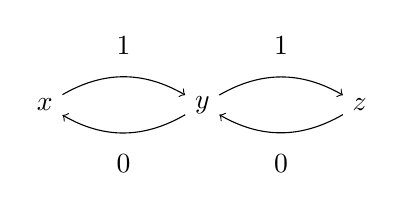
\begin{tikzpicture}
        \node (x) at (0,0) {$x$};
        \node (y) at (2,0) {$y$};
        \node (z) at (4,0) {$z$};
        \draw[->] (x) to [out=30,in=150] (y) node[xshift=-1cm, yshift=0.75cm]{$1$};
        \draw[->] (y) to [out=210,in=-30] (x) node[xshift=1cm, yshift=-0.75cm]{$0$};
        \draw[->] (y) to [out=30,in=150] (z) node[xshift=-1cm, yshift=0.75cm]{$1$};
        \draw[->] (z) to [out=210,in=-30] (y) node[xshift=1cm, yshift=-0.75cm]{$0$};
    \end{tikzpicture}
\end{center}
is represented by
\[P = \begin{pmatrix}
    0 & 1 & 0\\
    0 & 0 & 1\\
    0 & 1 & 0
\end{pmatrix}\] 

From $\P(X_1 = x_j \; | \; X_0 = x_i) = P_{ij}$, 
\begin{align*}
    \P(X_2 = x_j \; | \; X_0 = x_i) &= \sum_{k=1}^S \P(X_2 = x_j \; | \; X_0 = x_i, X_1 = x_k) \cdot \P(X_1 = x_k \; | \; X_0 = x_i)\\
    &= \sum_{k=1}^S \P(X_2 = x_j \; | \; X_1 = x_k) \cdot \P(X_1 = x_k \; | \; X_0 = x_i)\\
    &= \sum_{k=1}^S P_{kj} \cdot P_{ik}\\
    &= (P^2)_{ij}
\end{align*}
Then by induction, 
\[\P(X_n = x_j \; | \; X_0 = x_i) = (P^n)_{ij}\]

What if we want to calculate a state without a condition? 

We now define 
\[\mu = \begin{pmatrix}
    \P(X_0 = x_1)\\
    \P(X_0 = x_2)\\
    \vdots\\
    \P(X_0 = x_S)\\
\end{pmatrix}\]

So by the law of total probability, 
\begin{align*}
    \P(X_n = x_j) &= \sum_{j=1}^S \P(X_n = x_j \; | \; X_0 = x_i) \cdot \P(X_0 = x_i)\\
    &= \sum_{i=1}^S (P^n)_{ij}\cdot  \mu_i\\
    &= ((P^n)^T \mu)_j = (\mu^T P^n)_j
\end{align*}

\section{Lecture 13: Oct 24}
\subsection{Review}
$\{X_n\}_{n=0}^\infty$ is a HMC with state space $\mfX$ 
\[T_y(\omega) := \min \{n > 0: X_n(\omega) = y\}\]
\[\rho_{xy} := \P(T_y < \infty \; | \; X_0 = x)\]

A point $y$ is \emph{recurrent} if $\rho_{yy} = 1$ 

Recurrence is ``contagious'':
\[\begin{cases}
    \rho_{xx} = 1\\
    \rho_{yy} > 0
\end{cases} \implies \begin{cases}
    \rho_{yy} = 1\\
    \rho_{xy} = \rho_{yx} = 1
\end{cases} \]

The MC is \emph{irreducible} if $\rho_{xy} > 0$ for all $x, y \in \mfX$. By contagion, if there is one recurrent $y \in \mfX$, then all $x \in \mfX$ are recurrent. 

\textbf{Theorem:} If $\#\mfX < \infty$, the MC will have at least one recurrent point. Thus, all irreducible finite MCs are totally recurrent

\subsection{Directed Graphs}
With state space
\[\mfX = \{x_1, \dots,\; x_S\} \qquad S = \#\mfX\]

We have a transition matrix defined by 
\[P_{ij} = p(x_i, x_j)\]

Then, the \textbf{directed graph} $G(P) = (V, E)$ where $V$ is the set of vertices of the graph and $E$ is the set of directed edges between vertices.

The set of vertices is precisely the state space $\mfX$ and the set of directed edges are the connections from $x_i$ to $x_j$ for the points where $p(x_i, x_j) = P_{ij} > 0$

The transition matrix 
\[P = \begin{pmatrix}
    0.3 & 0 & 0 & 0 & 0.7 & 0 & 0\\
    0.1 & 0.2 & 0.3 & 0.4 & 0 & 0 & 0\\
    0 & 0 & 0.5 & 0.5 & 0 & 0 & 0\\
    0 & 0 & 0 & 0.5 & 0 & 0.5 & 0\\
    0.6 & 0 & 0 & 0 & 0.4 & 0 & 0\\
    0 & 0 & 0 & 0 & 0 & 0.2 & 0.8\\
    0 & 0 & 0 & 1 & 0 & 0 & 0
\end{pmatrix}\]
is represented by the graph
\begin{center}
    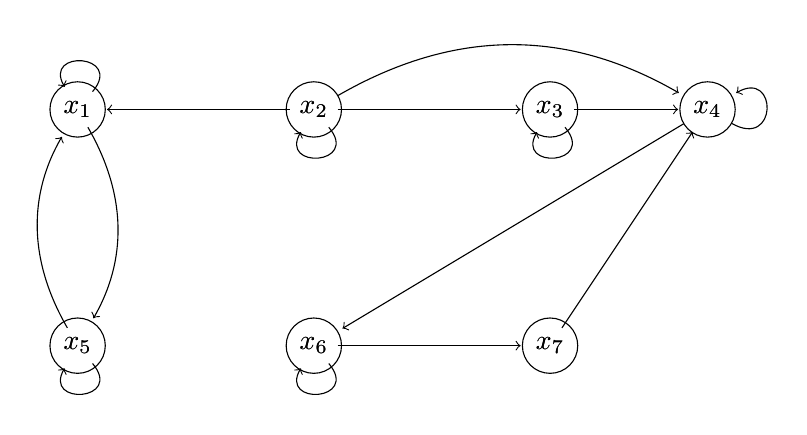
\begin{tikzpicture}
        \node (X1) at (0, 3){$x_1$};
        \node (X2) at (3, 3){$x_2$};
        \node (X3) at (6, 3){$x_3$};
        \node (X4) at (8, 3){$x_4$};
        \node (X5) at (0, 0){$x_5$};
        \node (X6) at (3, 0){$x_6$};
        \node (X7) at (6, 0){$x_7$};
    
        \draw (X1) circle (10pt) node{$x_1$};
        \draw (X2) circle (10pt) node{$x_2$};
        \draw (X3) circle (10pt) node{$x_3$};
        \draw (X4) circle (10pt) node{$x_4$};
        \draw (X5) circle (10pt) node{$x_5$};
        \draw (X6) circle (10pt) node{$x_6$};
        \draw (X7) circle (10pt) node{$x_7$};
    
        \draw[->, shorten >= 2pt] (X1) to [out=50,in=120, looseness=5] (X1);
        \draw[->, shorten >= 2pt] (X2) to [out=-50,in=-120, looseness=5] (X2);
        \draw[->, shorten >= 2pt] (X3) to [out=-50,in=-120, looseness=5] (X3);
        \draw[->, shorten >= 2pt] (X4) to [out=-30,in=30, looseness=5] (X4);
        \draw[->, shorten >= 2pt] (X5) to [out=-50,in=-120, looseness=5] (X5);
        \draw[->, shorten >= 2pt] (X6) to [out=-50,in=-120, looseness=5] (X6);

    
        \draw[->, shorten >= 4pt] (X1) to [bend left] (X5);
        \draw[->, shorten >= 4pt] (X5) to [bend left] (X1);
        \draw[->, shorten >= 2pt] (X2) -- (X1);
        \draw[->, shorten >= 2pt] (X2) -- (X3);
        \draw[->, shorten >= 2pt] (X2) to [bend left] (X4);
        \draw[->, shorten >= 2pt] (X3) -- (X4);
        \draw[->, shorten >= 2pt] (X4) -- (X6);
        \draw[->, shorten >= 2pt] (X7) -- (X4);
        \draw[->, shorten >= 2pt] (X6) -- (X7);
    \end{tikzpicture}
\end{center}


\textbf{Claim:} Let $\{X_n\}_{n=0}^\infty$ be an HMC. Its state space and transition matrix are $\mfX = \{x_1, \dots,\; x_S\}$ and $P$. The MC is irreducible if and only if $\forall x_i, x_j \in \mfX$, there x a directed edge from $x_1 \to x_j$ and a directed path from $x_j \to x_i$

\subsection{Stationary Distributions (SDs)}
Let $X_n \dot \sim \pi$ for large $n$: 
\[\pi(x) = \lim_{n\to \infty} \P(X_n = x)\]

By the Law of total probability, 
\begin{align*}
    \pi(x) &= \lim_{n\to \infty} \lim\P(X_n = x)\\
    &= \lim{n\to \infty} \sum_{y \in \mfX} \P(X_n = x \; | \; X_{n-1} = y) \cdot \P(X_{n-1} = y)\\
    &= \sum_{y \in \mfX} p(y, x) \cdot \lim_{n\to \infty} \P(X_{n-1} = y)\\
    &= \sum_{y \in \mfX} p(y, x) \cdot \pi(y)
\end{align*}

This leads us to a general formula: if $\pi(x) = \lim_{n\to\infty} \P(X_n = x)$ for all $x \in \mfX$ then, 
\[\pi(x) = \sum_{y\in \mfX} \pi(y) \cdot p(y, x)\]

\textbf{Definition:} Let $\{X_n\}_{n=0}^\infty$ be a HMC whose state space and transition probability are $\mfX$ and $P$. Suppose $\pi: \mfX \to \R$ is a PMF. Then $\pi$ is a \emph{stationary distribution} for the MC if 
\[\pi(x) = \sum_{y\in \mfX} \pi(y) \cdot p(y, x)\]

Define $\vec \pi = \begin{pmatrix}
    \pi(x_1)\\
    \vdots\\
    \pi(x_S)
\end{pmatrix}$. Then 
\[\pi(x) = \sum_{y\in \mfX} \pi(y) \cdot p(y, x) \iff \vec \pi = P^T \vec \pi\] 

\subsection{Existence of SDs}
\textbf{Simplex:}
\[\triangle = \{(p_1, p_2, \dots, p_S)^T : p_1 \geq 0, p_2 \geq 0 \dots,\; p_S \geq 0 \quad \text{and } \sum_{k=1}^S p_k = 1\}\]

In $3$-space, the simplex corresponds to the 2-d triangle between the vertices $(0, 0, 1), (0, 1, 0), (1, 0, 0)$

\textbf{Theorem:} If $\#\mfX < \infty$, the HMC has at least one stationary distribution, i.e. $\exists \vec \pi \in \triangle : \vec \pi = P^T \vec \pi$

    \emph{Proof:} Brouwer fixed-point Theorem (Algebraic topology) or Perron-Frobenius theorem (Linear algebra)

\subsection{Uniqueness of SDs}
\textbf{Theorem:} Let $\{X_n\}_{n=0}^\infty$ be a HMC with state space $\mfX$ and transition matrix $P$
\begin{enumerate}
    \item The MC has at least one SD 
    \item If the MC is irreducible, the SD is unique 
\end{enumerate}

\section{Lecture 14: Oct 26}
    \subsection{Review of Irreducibility}
        \textbf{Theorem:} If $\{X_n\}_{n=0}^\infty$ is a HMC with finite state space $\mfX$, then
        \begin{enumerate}
            \item The MC has at least one stationary distribution (SD) $\pi$
            \item If the the MC is irreducible the SD is unique and $\pi(x) > 0, \quad \forall x \in \mfX$ 
        \end{enumerate}

    \subsection{Aperiodicity}
        \textbf{Motivation:} The Ergodic theorem seeks to calculate the asymptotic distribution $\lim_{n\to\infty} \P(X_n = x)$ 

        \begin{align*}
            \lim_{n\to\infty} \P(X_n = x) &\overset{LTP}{=} \sum_{i=1}^S \lim_{n\to \infty} \P(X_n = x_j \; | \; X_0 = x_i) \cdot \P(X_0 = x_i)\\
            &= \sum_{i=1}^S \lim_{n\to \infty} (P^n)_{ij} \cdot \P(X_0 = x_i)
        \end{align*}
        So we need to caluclate $\lim_{n\to \infty} P^n$. 

        \textbf{Example:} 
        \[P = \begin{pmatrix}
            0 & 1\\
            1 & 0
        \end{pmatrix} \implies P^n = \begin{cases}
            I \quad \text{n even}\\
            P \quad \text{n odd}
        \end{cases}\] 
        So there is a ``periodic pattern'' to powers of $P$ and the limit does not exist. 

        \textbf{Definition:} Let $P$ be the transition matrix of an HMC whose state space is $\mfX = \{x_1, x_2, \dots,\; x_S\}$. Suppose the MC is irreducible. Let 
        \[I_i := \{n \geq 1: (P^n)_{ii} > 0\}\]
        and $d_i$ be the greatest common divisor of $I_i$. $d_i$ is the \emph{period} of $x_i$.


        In the example above, 
        \[I_1 = \{n \geq 1: (P^n)_{11} > 0\} = I_2 =  \{n \geq 1: (P^n)_{22} > 0\} = \{2, 4, 6, 8, \dots\}\]
        so $d_1 = d_2 = 2$

        And in fact that example represent the simple markov chain 
        \begin{center}
            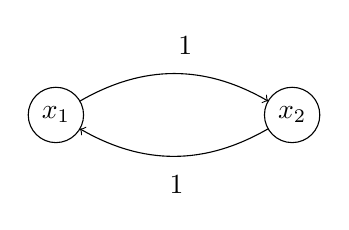
\begin{tikzpicture}
                \node (X1) at (0, 0) {$x_1$};
                \node (X2) at (3, 0) {$x_2$};

                \draw (X1) circle (10pt);
                \draw (X2) circle (10pt);
                
                \draw[->] (X1) to [bend left] (X2) node[xshift=-30pt, yshift=20pt] {$1$};
                \draw[->] (X2) to [bend left] (X1) node[xshift=35pt, yshift=-20pt] {$1$};
            \end{tikzpicture}
        \end{center}

        \textbf{Theorem:} $d_1 = d_2 = \dots = d_S$ 

        \emph{Proof:} Omitted

        \textbf{Definition:} the \emph{period} of the irreducible MC is $d:= d_1 = d_2 = \dots = d_S$

        \textbf{Remark:} We need the irreducibility constraint to ensure that $I_i \neq \emptyset$:irreducibility and finite state space means the MC is totally recurrent so 
        \[\infty = \sum_{n=1}^\infty \P(X_n = x_i \; | \; X_0 = x_i) = \sum_{n=1}^\infty (P^n)_{ii} \implies \exists i: (P^n)_{ii} > 0 \implies I_i \neq \emptyset\]

        \textbf{Definition:} an irreducible HMC is \emph{aperiodic} if its period is $d= 1$

    \subsection{1st Ergodic Theorem}
        \textbf{1st Ergodic Theorem:} Let $\{X_n\}_{n=0}^\infty$ be an HMC with finite state space. If the MC is irreducible and aperiodic, then 
            \[\lim_{n\to \infty} \P(X_n = x_j \; | \; X_0 = x_i) = \pi(x_j) \qquad \forall i, j \in \{1, 2, \dots, S\}\]
        where $\pi$ is the unique SD of the MC 

        \emph{Proof:} See lecture notes

        \textbf{Remark:} assuming that the state space was finite let us implicitly assume that the MC is recurrent (because one point is and it is irreducible) and that there is at least one SD (which is unique by irreducibility)

        \textbf{Corollary:} Under the conditions of the 1st Ergodic Theorem, 
        \[\lim_{n\to \infty} \P(X_n = x_j)  = \lim_{n\to \infty} \P(X_n = x_j \; | \; X_0 = x_i) = \pi(x_j)\]

        \emph{Proof:}
        \begin{align*}
            \lim_{n\to \infty} \P(X_n = x_j) &= \sum_{i=1}^n \left[\lim_{n\to\infty} \P(X_n = x_j \; | \; X_0 = x_i)\right] \cdot \P(X_0 = x_i)\\
            &=\sum_{i=1}^S \pi(x_j) \cdot \P(X_0 = x_i) \\
            &= \pi(x_j) \sum_{i=1}^S \P(X_0 = x_i)\\
            &= \pi(x_j) \cdot \P(x_i \in \mfX) = \pi(x_j)
        \end{align*}
        
        \textbf{Application:} Suppose we are interested in a distribution $\pi.$ If 
        \begin{enumerate}
            \item $\pi$ happens to be the SD of a MC $\{X_n\}_{n=0}^\infty$ 
            \item We know how to generate this MC
        \end{enumerate}
        Then $X_n \dot \sim  \pi$ when $n$ is large (so we can view $X_n$ as a RV drawn from $\pi$)

    \subsection{2nd Ergodic Theorem:} 
        \textbf{2nd Ergodic Theorem:} Let $\{X_n\}_{n=0}^\infty$ be an HMC with finite state space. If the MC is irreducible, for any $f: \mfX \to \R$, 
        $\sum_{x\in \mfX} \pi(x) \cdot \big\vert f(x_i)\big\vert < \infty$ where $\pi$ is the SD of the MC (unique by Irreducibility), then 
        \[\P\left(\omega \in \Omega: \lim_{n\to \infty} \frac{1}{n}\sum_{i=1}^n f(X_i(\omega)) = \sum_{x \in \mfX} \pi(x) \cdot f(x)\right) = 1\]

        \textbf{Application:} Suppose we are interested in computing $\sum_{x\in \mfX} \pi(x) \cdot f(x)$ (perhaps in the Ising Model of statistical mechanics, $\sum_{x\in \mfX} \pi(x) \cdot f(x) =$ ``average mangetization'').

        We can use an estimator:
        \[\hat v_n = \frac{1}{n}\sum_{i=1}^n f(X_i) \approx v\]

    \subsection{Markov Chain Monte Carlo} 
        \textbf{Problem:} Given a distribution $\pi$, we want to derive a transition matrix $P$ such that $\pi$ is the SD of $P$ 
        
        Note that, in general, this is a much harder problem than finding $\pi$ given $P$!

       \textbf{Solutions:}
       \begin{itemize}
        \item Method 1: Metropolis-Hastings Algorithm
        \item Method 2: Gibbs Sampling
       \end{itemize}

\section{Lecture 15: Oct 31}
    \subsection{Review}
        \textbf{Ergodic Theorem:} Let $\{X_n\}_{n=0}^\infty$ be an HMC on finite state space $\mfX$. Then, we have 
        \begin{enumerate}
            \item The MC is recurrent (all $x \in \mfX$) are recurrent
            \item The MC has a unique stationary distribution $\pi: \mfX \to \R$ 
            \item $X_n \sim \pi$ at large $n$. i.e., $\lim_{n\to \infty}\P(X_n = x) = \pi(x)\quad \forall x\in \mfX$
            \item 
            \[\P(\{\omega \in \Omega: \lim_{n\to \infty} \frac{1}{n}f(X_i(\omega)) = \E_{\pi} f(X)\}) = 1\]
            where $f: \mfX \to \R$ and $\E_{\pi} f(X) = \sum_{x \in \mfX} \pi(x) \cdot f(x)$
        \end{enumerate}

        This last statement is exactly like the Law of Large Numbers except in the LLN, the RVs are required to be iid. Here, they just need to be elements of the same Markov Chain.

    \subsection{Markov Chain Monte Carlo}
        Suppose we are given a distribution $\pi: \mfX \to \R$ and have derived a transition probability $p: \mfX \times \mfX \to \R$ satisfying 
        \[\pi(x) = \sum_{y\in \mfX} \pi(y) \cdot p(y, x) \quad \forall x\in \mfX\]
        (i.e. it is a stationary distribution) 
        
        Then we can use the following algorithm to generate a sequence of RV $\{X_n\}_{n=0}^\infty$ that form a MC with transition probability $p$ and SD $\pi$: 
        \begin{verbatim}
            Initialize X0

            for n = 1, 2, ...
        \end{verbatim}
        \hspace*{2in} $X_n \sim p(X_{n-1}, \cdot)$
        \begin{verbatim}
            end for
        \end{verbatim}

        \textbf{Remarks:}
        \begin{enumerate}
            \item $p(X_{n-1}, \cdot)$ is a two-variable function with one input fixed. Thus the algorithm step corresponds to generating $X_n \sim p_{X_{n-1}}(y)$ (generating an RV from a PMF)
            \item 
            \begin{align*}
                p(x, y) &\geq 0\\
                \P(X_1 = y \; | \; X_0 = x) &\geq 0
            \end{align*}
        \end{enumerate}

        \textbf{Goals:}
        \begin{enumerate}
            \item $X \dot \sim \pi$
            \item Approx $\sum_{x\in \mfX} \pi(x) \cdot f(x)$
        \end{enumerate}

        \textbf{Problem:} in most applications, the dimensionality of $\pi(\vec x)$ is very large 

    \subsection{Summaries of Pictures}
        We define a \emph{picture} as a vector $x = (x^{(1)}, x^{(2)}, \dots,\; x^{(d)})$ where each $x^{(i)}$ is a \emph{pixel}. 

        A \emph{random picture} is a random vector $X = (X^{(1)}, X^{(2)}, \dots,\; X^{(d)}) \sim \pi$. 

        In general, it is infeasible to generate a random picture from $\pi$, but we can generate an HMC $\{X_n\}_{n=0}^\infty$ whose SD is $\pi$ so $X_n \dot \sim \pi$.

        Then say we have $f: \R^d \to \R$ which gives a \emph{summary of the picture}. For example, 
        \[f(x) = \frac{1}{d}\sum_{i=1}^d x^{(i)} \]

        Further, the probability that a particular picture $x$ is observed is $\pi(x): \mfX \to \R$. 

        So the average summary of a pictures is 
        \[v = \sum_{x \in \mfX} \pi(x) \cdot f(x)\]
        
        For a 256x256 picture, this sum would have $2^{65536}$ terms, so this obviously cannot be calculated theoretically. 

        However, using MCMC, we can create an estimator for $v$ (assuming we have a HMC with SD $\pi$):
        \[\hat v = \frac{1}{n}\sum_{i=1}^n f(X_i) \approx v\]

        The process of creating that MC from $\pi$ is the central topic of MCMC theory.

\section{Lecture 16: Nov 2 }  
    \subsection{Review of the MCMC}
        Our goal is to generate random numbers from a given distribution $\pi$. If we find the transition probability of an irreducible and aperiodic HMC and sample via $X_n \sim p(X_{n-1}, \cdot)$, then $\{X_n\}_{n=0}^\infty$ will be an HMC whose SD is $\pi$ and thus the sample average will converge to the SD by the ergodic theorem. Thus, sampling from $p$ will give us random variables from $\pi$. 

    \subsection{Metropolis Algorithm (1953)}
        Assume we are given a function $\pi: \mfX \to \R$, satisfying $\pi(x) > 0 \quad \forall x \in \mfX$

        We choose a $q: \mfX \times \mfX \to \R$ satisfying 
        \begin{enumerate}
            \item $q$ is the transition probability of an HMC
            \item That MC is irreducible and aperiodic 
            \item $q$ is symmetric: $q(x, y) = q(y, x) \quad \forall x, y \in\mfX$
            \item For each fixed $x$, $q(x, \cdot) = q_x(y)$ is a PMF from which we know how to generate RVs in an efficient way
        \end{enumerate}

        Then the Metropolis Algorithm defines $p(x, y)$ by 
        \[p(x, y) := \begin{cases}
            q(x, y) \cdot \min\{1, \frac{\pi(y)}{\pi(x)}\} \qquad x \neq y\\
            1 - \sum_{\xi \in \mfX: \xi \neq x} p(x, \xi) \qquad x = y
        \end{cases}\]

        \textbf{Remark:} Because of the ratio $\frac{\pi(y)}{\pi(x)}$ in the Metropolis Algorithm, we do not need the exact formula of $\pi$ -- just the formula up to a constant which will be cancelled. 

        \textbf{Theorem:} Let $q$ be the transition probability of an irreducible and aperiodic HMC. Suppose $q$ is symmetric. 

        If $\{X_n\}_{n=0}^\infty$ is an HMC whose transition probability is the $p$ of the Metropolis algorithm, then the MC is irreducible and aperiodic and its SD is $\pi$

        Thus, by the Ergodic Theorem, $X_n \dot\sim \pi$ (for large $n$) so 
        \[\lim_{n\to \infty} \P(X_n = x) = \pi(x) \quad \forall x\]

        Further, we can define an estimator 
        \[\hat v_n = \frac{1}{n}\sum_{i=1}^n f(X_i) \approx \sum_{x\in \mfX} \pi(x) \cdot f(x) = v\]

        \subsection{Algorithmic Metropolis}
            \begin{verbatim}
                Inputs: pi, q, x0
                Outputs: X[0], X[1], X[2], ..., X[n]

                Init X[0] <-- x0;
                for n = 1, 2, 3, ...
                    X' ~ q(X[n-1], ?);
                    r <-- pi(X')/pi(X[n-1]);
                    y ~ Bernoulli(min(1, r));
                    X[n] <-- y * X' + (1 - y)*X[n-1]
                end 
            \end{verbatim}

        \subsection{Example: 2-dim Multivariate Normal Distribution}
            \begin{align*}
                \pi(x_1, x_2) &= c \cdot \exp\left(-\frac{1}{2}(x_1, x_2) \begin{pmatrix}
                    1 & 0.8\\
                    0.8 & 1
                \end{pmatrix}^{-1} \begin{pmatrix}
                    x_1\\x_2
                \end{pmatrix}\right)\\
                &= N\left(\begin{pmatrix}
                    0\\0
                \end{pmatrix}, \begin{pmatrix}
                    1 & 0.8\\
                    0.8 & 1
                \end{pmatrix}\right)\\
                q(x, y) &= q((x_1, x_2), (y_1, y_2))\\
                &= \left(\frac{2\pi}{25}\right)^2 \cdot \exp\left(-\frac{25}{2}\left[(x_1 - y_1)^2 + (x_2 - y_2)^2\right]\right)\\
                q_{x_1}(y) &= N\begin{pmatrix}
                    x_1\\x_2
                \end{pmatrix}, \begin{pmatrix}
                    \sigma^2 & 0\\
                    0 & \sigma^2
                \end{pmatrix}\\
                &= N\left(\begin{pmatrix}
                    x_1\\x_2
                \end{pmatrix}, \begin{pmatrix}
                    \frac{1}{25} & 0\\
                    0 & \frac{1}{25}
                \end{pmatrix}\right)
            \end{align*}

            Note that this simulation is very sensitive to changes in $\sigma$. When $\sigma$ is large, for example, $r = \frac{\pi(X*)}{\pi(X_{n-1})}$ tends to be small so $Y$ tends to $0$ so 
            \[X_n = Y\cdot X* + (1- y)X_{n-1} = X_{n-1}\]
            
            When $\sigma$ is very small, $\text{dist}(X*, X_{n-1})$ is small so $r \to 1$, $Y \to 1$, and $X_n = X*$. 

        \subsection{Metropolis-Hastings Algorithm (1970)}
            Note that sometimes, we cannot choose symmetric $q$ so we need a different formula: 
            \[p(x, y) = \begin{cases}
                q(x, y)\cdot \min\{1, \frac{\pi(y) \cdot q(y,x)}{\pi(x) \cdot q(x, y)}\} \qquad x\neq y, \; q(x, y) \neq 0\\
                0 \hspace*{2in} x\neq y, q(x, y) = 0\\
                1 - \sum_{\xi \in \mfX: \xi\neq x} p(x, \xi) \qquad \qquad x = y
            \end{cases}\]

            \textbf{Theorem:} Let $\{X_n\}_{n=0}^\infty$ be an HMC whose transition prob is this $p$. Then, the MC is irreducible, aperiodic, and has SD $\pi$.

\section{Lecture 17: Nov 7}
    \subsection{Choosing $q$ in the Metropolis Algorithm}  
        Recall that both the Metropolis and Metropolis-Hastings algorithm require a known function $q(x, y)$ from which to sample new RVs and which is used to define $p$. 
        
        Now matter the choice of $q$, $\lim_{n\to\infty} \P(X_n = x) = \pi(x)$ but the rate of convergence is very strongly dependent on the choice of $q$.

        Specifically, the convergence rates depend on the eigenvalues of 
        \[P = (p(x_i, x_j))_{1 \leq i, j \leq n}\]

        Unfortunately, the specific relationship is outside the scope of this course. 

        In applications, we 
        \begin{enumerate}
            \item try different $q$
            \item for each $q$, generate a ``long chain'' $\{X_n\}_{n=0}^N$ for large $N$
        \end{enumerate}

        If you do not want to choose $q$, use Gibbs Sampling instead of MCMC. 

    \subsection{Gibbs Sampling (1984)}
        \textbf{2-dim Gibbs Sampling ($\pi(\xi_1, \xi_2)$):}
            Let $\pi(\xi_1, \xi_2) > 0 \quad \forall \xi_1, \xi_2$. We then define two marginal distributions
            \begin{align*}
                \pi_1(\xi_1) &= \sum_{\xi_2} \pi(\xi_1, \xi_2)\\
                \pi_2(\xi_2) &= \sum_{\xi_1} \pi(\xi_1, \xi_2)
            \end{align*}
            and condtional distributions
            \begin{align*}
                \pi_{1 \; | \; 2}(\xi_1 \; | \; \xi_2) &= \frac{\pi(\xi_1, \xi_2)}{\pi_2(\xi_2)} \\
                \pi_{2 \; | \; 1}(\xi_2 \; | \; \xi_1) &= \frac{\pi(\xi_1, \xi_2)}{\pi_1(\xi_1)} 
            \end{align*}

            Further, since $\pi(x_1, \xi_2) >0$, all four distributions will be positive.
            
            Now let $x = (\xi_1, \xi_2)$ and $y = (\eta_1, \eta_2)$. Then 
            \begin{align*}
                p(x, y) &:= \pi_{1\; | \;2}(\eta_1 \; | \; \xi_2) \cdot \pi_{2 \; | \; 1}(\eta_2 \; | \; \eta_1)\\
                &= \frac{\pi(\eta_1, \xi_2)}{\pi_2(\xi_2)} \cdot \frac{\pi(\eta_1, \eta_2)}{\pi_1(\eta_1)}
            \end{align*}


        \textbf{Explanation:}
        
        Let $\{X_n\}_{n=0}^\infty$ be the HMC whose transition probability is $p$

        \emph{Claim 1:} The MC is irreducible

        \emph{Proof:} $0 < p(x, y) = \P(X_1 = y \; | \; X_0 = x) \leq \P(T_y < \infty \; | \; X_0 = x) = \rho_{xy} \qed$

        \emph{Claim 2:} The MC is aperiodic. 

        \emph{Proof:} We assume $\mfX = \{x_1, x_2, \dots,\; x_S\}$ so 
        \[P = (p(x_i, x_j))_{1 \leq i, j \leq S}\]
        and $(P)_{ii} = (P^1)_{ii} = p(x_i, x_i) > 0$. So $1 \in I_i \implies \gcd(I_i) = 1$. $\qed$. 

        \emph{Claim 3:} The SD of the MC is $\pi$. 

        \emph{Proof:} $x = (\xi_1, \xi_2)$ and $y = (\eta_1, \eta_2)$. 
        \begin{align*}
            \sum_x \pi(x) \cdot p(x, y) &= \sum_{\xi_2} \sum_{\xi_1} \pi(\xi_1, \xi_2) \cdot \frac{\pi(\eta_1, \xi_2)}{\pi_2(\xi_2)} \cdot \frac{\pi(\eta_1, \eta_2)}{\pi_1(\eta_1)}\\
            &= \sum_{\xi_2} \left(\sum_{\xi_1} \pi(\xi_1, \xi_2)\right) \cdot \frac{\pi(\eta_1, \xi_2)}{\pi_2(\xi_2)} \cdot \frac{\pi(\eta_1, \eta_2)}{\pi_1(\eta_1)}\\
            &= \sum_{\xi_2} \pi_2(\xi_2) \cdot \frac{\pi(\eta_1, \xi_2)}{\pi_2(\xi_2)} \cdot \frac{\pi(\eta_1, \eta_2)}{\pi_1(\eta_1)}\\
            &= \sum_{\xi_2} \pi(\eta_1, \xi_2)\cdot \frac{\pi(\eta_1, \eta_2)}{\pi_1(\eta_1)}\\
            &= \pi_1(\eta_1) \cdot \frac{\pi(\eta_1, \eta_2)}{\pi_1(\eta_1)}\\
            &= \pi(\eta_1, \eta_2)\\
            &= \pi(y)
        \end{align*}

\section{Lecture 18: Nov 9}
    \subsection{Notation}
        Let $\pi(\xi_1, \xi_2, \dots,\; \xi_d)$ be a PMF on d-space. 

        We can create a marginal distribution, 
        \[\pi_{-i}(\xi_1, \dots, \; x_{i-1}, \xi_{i+1}, \dots,\; \xi_d) = \sum_{\xi_i} \pi(\xi_1, \dots,\; \xi_i, \dots,\; \xi_d)\]

        And using the joint distribution and marginal distribution, we have a conditional distribution 
        \[\pi_{i|-i}(\xi_i \; | \; \xi_1, \dots,\; \xi_{i-1}, \xi_{i+1}, \dots,\xi_d)\]

        \textbf{Remark:} this is a very natural extension of what we did in the 2-d Gibbs Sampling case. 

    \subsection{2-dim Gibbs Sampler} 
        \textbf{Inputs:} a given distribution $\pi(\xi_1, \xi_2)$ and an initial state $x_0 = (\xi_1, \xi_2)$

        \textbf{Output:} a HMC $\{X_n = (\xi_1^{(n)}, \xi_2^{(n)})\}_{n=0}^\infty$

        \textbf{Algorithm:} 
            \begin{verbatim}
                for n = 1, 2, ...
            \end{verbatim}
            \begin{center}
                Generate $\xi_1^{(n)} \sim \pi_{1\; | \;2}(\circ \; | \; \xi_2^{(n-1)})$

                Generate $\xi_2^{(n)} \sim \pi_{2\; | \;1}(\circ \xi_1^{(n-1)} \; | \;)$

                $X_n = (\xi_1^{(n)}, \xi_2^{(2)})$
            \end{center}
            \begin{verbatim}
                end for
            \end{verbatim}

    \subsection{d-Dimensional Gibbs Sampler}
        \textbf{Inputs:} Given $\pi(\xi_1, \xi_2, \dots,\; \xi_d)$, and $x_0 = (\xi_1^{(0)}, \xi_2^{(0)}, \dots,\; \xi_d^{(0)})$

        \textbf{Outputs:} a HMC $\{X_n = (\xi_1^{(n)}, \dots, xi_d^{(n)})\}_{n=0}^\infty$

        \textbf{Algorithm:}
        \begin{lstlisting}
        X0 <-- x0
        for n = 1, 2, 3, ...
            Generate $\xi_1^{(n)} \sim \pi_{1\; | \;-1}(\circ \; | \; \xi_2^{(n-1)}, \dots,\; \xi_d^{(n-1)})$
        
            for j = 2, 3, ..., d
                Generate  $\xi_j^{(n)} \sim \pi_{j\; | \;-j}(\circ \; | \; xi_1^{(n)}, \dots,\; \xi_{j-1}^{(n)}, \xi_{j+1}^{(n- 1)}, \dots,\; \xi_{d}^{(n-1)})$
            end for

            $x_n \longleftarrow (\xi_1^{(n)}, \dots,\; \xi_d^{(n)})$
        end for
        \end{lstlisting}

        \textbf{Problem:} Generating 
        \begin{align*}
            \xi_j &\sim \pi_{j \; | \; -j}(\xi_j \; | \; \xi_1, \dots, \; \xi_{j-1}, \xi_{j+1}, \dots,\; \xi_d)\\
            &= \frac{\pi(\xi_1, \dots, \; \xi_{j-1}, \xi_j, \xi_{j+1}, \dots,\; \xi_d)}{\sum_{\xi_j}\pi(\xi_1, \dots, \; \xi_{j-1}, \xi_j, \xi_{j+1}, \dots,\; \xi_d)}
        \end{align*}
        is generally infeasible. 

        This method only works if $\pi$ is a Gibbs Random Field. 

    \subsection{Ising Model}
        The most famous GRF is the Ising Model of statistical mechanics.

        We construct an $n$-by-$n$ lattice where each vertex has a magnetic monopole. $s_i \in \{-1, 1\}$ where $-1$ corresponds to a South pole and $+1$ to a North pole. 

        \begin{center}
            \begin{tikzpicture}[clip=false]
                \begin{axis}[hide axis, xmin=0,xmax=3,ymin=0,ymax=3]
                    \draw (axis cs: 0, 0) -- (axis cs: 3, 0) node{0};
                    \draw (axis cs: 0, 1) -- (axis cs: 3, 1) node{1};
                    \draw (axis cs: 0, 2) -- (axis cs: 3, 2) node{2};
                    \draw (axis cs: 0, 3) -- (axis cs: 3, 3) node{3};
                    
                    \draw (axis cs: 0, 0) -- (axis cs: 0, 3) node{0};
                    \draw (axis cs: 1, 0) -- (axis cs: 1, 3) node{1};
                    \draw (axis cs: 2, 0) -- (axis cs: 2, 3) node{2};
                    \draw (axis cs: 3, 0) -- (axis cs: 3, 3) node{3};

                    \draw (axis cs: 2, 2) circle (3pt) node[xshift=0.3cm, yshift=-0.3cm]{$i$};
                \end{axis}
            \end{tikzpicture}
        \end{center}

        The \emph{magnetic structure} of the lattice is 
        \[\vec s = (s_1, s_2, \dots,\; s_{N^2})\]
        
        \[f(\vec s) = \frac{1}{N^2} \sum_i s_i\]

        \begin{itemize}
            \item If $\big\vert f(\vec s) \big\vert = 0$ the lattice is not magnetic because the north and south poles cancel.
            \item If $\big\vert f(\vec s)\big\vert > 0$ the lattice is magnetic
        \end{itemize}

        \textbf{Problem:} What if $\vec s$ is not deterministic. i.e., $\vec s = \pi(s_1, \dots, \; s_{N^2})$? 

        Each $\vec s$ is associated with an energy value 
        \[H_N(\vec s) = - \sum_{\langle i, j\rangle} s_i s_j\] 

        \begin{itemize}
            \item If $s_i = s_j \implies s_i s_j = 1 \implies \text{low energy}$
            \item If $s_i \neq s_j \implies s_i s_j = -1 \implies \text{high energy}$
        \end{itemize}

        \textbf{The Ising Model:}  
        \[\pi_{N, \beta}(\vec s) = \frac{1}{Z(\beta)} \exp(-\beta \cdot H_N(\vec s))\]
        where $\beta = 1/T$ (the temperature) and $Z(\beta)$ is the partition function 
        \[Z(\beta) = \sum_{\vec s} \exp\{-\beta H_N(\vec s)\}\] 

        and 
        \[\E_{\pi_{N, \beta}}((f(\vec s))) = \sum_{\vec s} \pi_{N, \beta}(\vec s) \cdot \underbrace{\bigg\vert \frac{1}{N^2} \sum_i s_i \bigg\vert}_{m_N(\beta)}\] 

        In most applications, each vertex denotes an atom and $N \approx \infty$ so 
        \[m(\beta) = \lim_{N\to \infty} m_N(\beta)\]

        \begin{itemize}
            \item If $m(\beta) > 0$, the ``infinitely large'' lattice is magnetic
            \item If $m(\beta) = 0$, the lattice is not magnetic
        \end{itemize}

        Note that $\beta$ is defined by a temperature. When $\beta = \beta^*$, the \emph{Curie Temperature},  t certain materials begin to lose their permanent magnetic properties. 
        \[\beta^* = \frac{\log(1 + \sqrt{2})}{2}\]

\section{Lecture 19: Nov 14}
    \subsection{Ising Model}
        We have an $N$-by-$N$ lattice with $N^2$ vertices. Each vertex $i$ is associated with a binary $s_i \in \{-1, 1\}$. Let $\vec s = (s_1, s_2, \dots,\; s_{N^2})$. 

        Then $\mfX$ is the collection of all possible vectors $\vec s$: 
        \[\mfX = \underbrace{\{-1, 1\}\times \{-1, 1\} \times \dots \times \{-1, 1\}}_{N^2 \text{ times}} \implies \#\mfX = 2^{N^2}\]

        Let $\pi: \mfX \to \R$ be a PMF on $\mfX$ expressed by 
        \[\pi_{N, \beta}(\vec{s}) = \frac{1}{Z(\beta)}\exp(-\beta \cdot H_N(\vec s))\]
        where 
        \[H_N(\vec s) = -\sum_{\langle i, j\rangle} s_i s_j\]
        is an energy function (the bracket notation indicates $i, j$ are neighbours i.e., there is an edge between them), $\beta = \frac{1}{T}$ where $T$ is the temperature, and ($\beta > 0$)
        \[Z(\beta) = \sum_{\vec s} \exp(-\beta \cdot H_N(\vec s))\]

        Let $f: \mfX \to \R$ be a different function on the state space giving the average value of entries in a vector:
        \[f(\vec s) = \frac{1}{N^2}\sum_{i=1}^{N^2}s_i\]

        Most often in applications, we are interested in the characteristics of the full state space -- not any particular vector. So we take 
        \[m_N(\beta) = \sum_{\vec s \in \mfX} \pi_{N, \beta}(\vec s) \cdot \abs{f(\vec s)} = \E_{\pi_{N, \beta}}\abs{f(\vec s)}\]

        Further, in physics we generally care about a huge amount of particles:
        \[m(\beta) = \lim_{N\to \infty} m_N(\beta)\]
        (this is the \emph{magnetization} of the lattice)

        \textbf{Remark:} $m(\beta)$ is a function of $\beta$ and is called the \emph{magnetization curve}. It looks like:

        \begin{center}
            \begin{tikzpicture}
                \begin{axis}[ticks=none, xlabel=$\beta$, ylabel=$m(\beta)$, axis lines=middle, xmin=0, xmax=6, ymin=-0.5, ymax=2.5]
                    \addplot[samples=100, smooth, thick, blue] {tanh(x-4)+1};
                    \node at (axis cs: 1.3, 0.1) {$\beta^*$};
                \end{axis}
            \end{tikzpicture}
        \end{center}

        Theoretically, 
        \[\beta^* = \frac{\log(1 + \sqrt 2)}{2}\]
        but the calculation of this value was worthy of a Nobel Prize. 

        We will approximate $\beta^*$. To get $\beta^*$, we need $m(\beta)$. When $N$ is very large, 
        \[m(\beta) \approx m_N(\beta) = \sum_{\vec s} \pi_{N,\beta} \cdot \abs{f(\vec s)} = \E_{\pi_{N, \beta}} \abs{f(\vec s)}\]

    \subsection{Using the MCMC}
        Suppose we have an HMC $\{X_n\}_{n=0}^\infty$ on the state space $\mfX$ which is irreducible, aperiodic, and its SD is $\pi$. 
        
        By the Ergodic Theorem, 
        \[\lim_{n\to \infty} \frac{1}{n}\sum_{i=1}^n \abs{f(X^{(i)})} = \E_{\pi_{N, \beta}}\abs{f(X^{(i)})} = m_N(\beta)\]

        So when both $N$ and $n$ are large, 
        \[m(\beta) \approx m_N(\beta) \approx \frac{1}{n}\sum_{i=1}^n \abs{f(X^{(i)})}\]

        Thus, with only a small reduction in accuracy do to the approximation, we have reduced a Nobel-Prize level question into a simple high-school level average. 

        \textbf{Problem:} How do we construct an HMC $\{X_n\}_{n=0}^\infty$ with SD $\pi$?

        \textbf{Solution:} Gibbs Sampling 

    \subsection{The Conditional Distribution}
        The central principle of Gibbs sampling is drawing for a specific conditional distribution, $\pi_{i \; | \; -i}$.

        \emph{Note on notation:} Let $\pi = \pi_{N, \beta}$. 

        Then we have a PMF $\pi(s_1, \dots,\; s_j, \dots,\; s_{N^2})$ and we can define a conditional distribution
        \[\pi_{j \; | \; -j}(s_j \; | \; s_1, \dots,\; s_{j-1}, s_{j+1}, \dots,\; s_{N^2}) = \frac{\pi(s_1, \dots,\; s_j, \dots,\; s_{N^2})}{\sum_{s_j} \pi(s_1, \dots,\; s_j, \dots,\; s_{N^2})}\]

        Since we are applying this specifically to the Ising Model, we have an expression for $\pi$ we can use to simplify the above. Focus on a single vertex $j$. Then from the Ising model, 
        \[H_N(\vec s) = -\sum_{\brak{i,j}} s_i s_j \implies H_N(\vec s) = -s_j s_{j, l} - s_j s_{j, r} - s_j s_{j, u} - s_j s_{j, d} - \sum_{\brak{k, l}: k, l \neq j} s_{kl}\]

        We define $\mathcal{N}(j) = \{jl, jr, ju, jd\}$ to be the (neighborhood of $j$) so 
        \[H_N(\vec s) = -\sum_{j' \in \mathcal{N}(j)} s_j s_{j'} - \sum_{\brak{k, l}: k, l \neq j} s_k s_l\]

        This gives a new expression for $\pi$:
        \[\pi(\vec s) = \frac{1}{Z(\beta)} \cdot \exp(\beta\cdot H_N(\vec s)) = \frac{1}{Z(\beta)} \cdot \exp\left(-\beta \sum_{j' \in \mathcal{N}(j)} s_j s_{j'}\right) \cdot \exp\left(-\beta \sum_{\brak{k, l}: k, l \neq j} s_k s_l\right)\]
        which we can plug in to the conditional distribution:
        \begin{align*}
            \pi_{j \; | \; -j}(s_j \; | \; s_1, \dots,\; s_{j-1}, s_{j+1}, \dots,\; s_{N^2}) &= \frac{\pi(s_1, \dots,\; s_j, \dots,\; s_{N^2})}{\sum_{s_j} \pi(s_1, \dots,\; s_j, \dots,\; s_{N^2})}\\
            &= \frac{ \frac{1}{Z(\beta)} \cdot \exp\left(-\beta \sum_{j' \in \mathcal{N}(j)} s_j s_{j'}\right) \cdot \exp\left(-\beta \sum_{\brak{k, l}: k, l \neq j} s_k s_l\right)}{\sum_{s_j}  \frac{1}{Z(\beta)} \cdot \exp\left(-\beta \sum_{j' \in \mathcal{N}(j)} s_j s_{j'}\right) \cdot \exp\left(-\beta \sum_{\brak{k, l}: k, l \neq j} s_k s_l\right)}\\
            &= \frac{\exp\left(-\beta \sum_{j' \in \mathcal{N}(j)} s_j s_{j'}\right)}{\sum_{s_j \in \{-1, 1\}} \exp\left(-\beta \sum_{j' \in \mathcal{N}(j)} s_j s_{j'}\right)}\\
            &= \frac{\exp\left(-\beta \sum_{j' \in \mathcal{N}(j)} s_j s_{j'}\right)}{\exp\left(\beta \sum_{j' \in \mathcal{N}(j)} s_{j'}\right) + \exp\left(-\beta \sum_{j' \in \mathcal{N}(j)} s_{j'}\right)}
        \end{align*}

        For simplicity, let 
        \begin{align*}
            a = \exp\left(\beta \sum_{j' \in \mathcal{N}(j)} s_{j'}\right)\\
            b = \exp\left(-\beta \sum_{j' \in \mathcal{N}(j)} s_{j'}\right)
        \end{align*}

        Then we have two cases for $\pi$:
        \begin{align*}
            \pi_{j  | -j}(1 \; | \; \dots) &= \frac{b}{a + b}\\
            \pi_{j  | -j}(-1 \; | \; \dots) &= \frac{a}{a + b}
        \end{align*}

        i.e., 
        \begin{align*}
            \P(s_j = -1) = \frac{a}{a + b}\\
            \P(s_j = 1) = \frac{b}{a + b} 
        \end{align*}

    \subsection{Using Gibbs}
        Now we want to generate $X^{(n)} \sim \pi_{j\vert -j}(? \; | \; s_1, \dots,\; s_{j-1}, s_{j+1}, \dots,\; s_{N^2})$.

        \begin{enumerate}
            \item Compute 
            \[a = \exp\left(\beta \sum_{j' \in \mathcal{N}(j)} s_{j'}\right)\]
            \item Compute 
            \[b = \exp\left(-\beta \sum_{j' \in \mathcal{N}(j)} s_{j'}\right)\]
            \item Compute
            \[p = \frac{b}{a + b}\]
            \item Generate 
            \[Z \sim \text{Bernoulli}(p)\]
            \item Transform $Z \in \{0, 1\}$ to $s_j \in \{-1, 1\}$:
            \[s_j = 2Z - 1\]
        \end{enumerate}
       
        Then generate $\{X^{(n)} = (X_1^{(n), X_2^{(n)}, \dots,\; X_{N^2}^{(n)}})\}_{n=1}^\infty$. 
        
        By the Ergodic Theorem, $X^{(n)} \dot \sim \pi_{N, \beta}$ 

\section{Lecture 20: Nov 16}
    \subsection{Graphs}
        \textbf{Definition:} A graph is an ordered pair $G = (V, E)$ where 
        \begin{enumerate}
            \item $V$ is the collection of vertices 
            \item $E$ is the collection of (undirected) edges 
        \end{enumerate}

        \textbf{Remarks:}
        \begin{itemize}
            \item An edge connecting vertices $i$ and $j$ is denoted $(i, j)$
            \item We are focused on undirected graphs so $(i, j) = (j, i)$ 
            \item For each edge $(i, j) \in E$, we require $i \neq j$
        \end{itemize}

        \textbf{Definition:} Let $G = (V, E)$ be a graph.
        \begin{enumerate}
            \item two vertices $i$ and $j$ are \emph{adjacent} if $(i, j) \in E$.
            \item Let $i \in V$. The \emph{neighborhood} of $i$ is 
            \[\mathcal{N}(i) = \{j \in V: (i, j) \in E\}\]
        \end{enumerate}


        \textbf{Example:}
        \begin{center}
            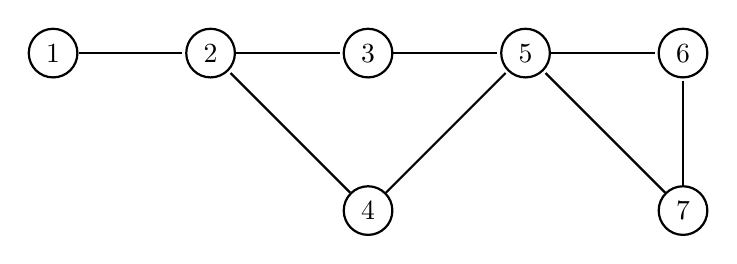
\begin{tikzpicture}[shorten >=1pt, auto, node distance=2cm, thick, main node/.style={circle,draw}]

                \node[main node] (1) {1};
                \node[main node] (2) [right of=1] {2};
                \node[main node] (3) [right of=2] {3};
                \node[main node] (4) [below of=3] {4};
                \node[main node] (5) [right of=3] {5};
                \node[main node] (6) [right of=5] {6};
                \node[main node] (7) [below of=6] {7};
    
                \path[every node/.style={font=\sffamily\small}]
                    (1) edge node [left] {} (2)
                    (2) edge node [right] {} (3)
                    (3) edge node [right] {} (5)
                    (5) edge node [right] {} (6)
                    (4) edge node [below] {} (2)
                    (4) edge node [below] {} (5)
                    (7) edge node [below] {} (5)
                    (7) edge node [below] {} (6);
            \end{tikzpicture}
        \end{center}
        
        This picture shows a graph $G$. $\mathcal{N}(5) = \{3, 4, 6, 7\}$. 

        \textbf{Definition:} Let $G = (V, E)$ be a graph. 
        \begin{enumerate}
            \item A subset $c \subseteq V$ is called a \emph{clique} if any pair of vertices in $c$ are adjacent. 
            \item Let $\mathcal{C}(G)$ be the collection of all cliques in $G$.
        \end{enumerate}

        \textbf{Convention:} for each $i \in V$, the singleton $\{i\}$ is a clique

        In the graph above, the cliques are: 
        \begin{itemize}
            \item $\{1\}, \{2\}, \{3\}, \{4\}, \{5\}, \{6\}, \{7\}$
            \item $\{1, 2\}, \{2, 3\}, \{3, 5\}, \{5, 6\}, \{4, 2\}, \{4, 5\}, \{7, 5\}, \{7, 6\}$
            \item $\{5, 6, 7\}$
        \end{itemize}

        \textbf{Notation:} 
        \begin{itemize}
            \item Let $G = (V, E)$ be a graph with $V = \{1, \dots,\; d\}$ and $x = (x_1, \dots,\; x_d)^T$ a vector in the product space $\mfX = \mfX_1 \times \dots \times \mfX_d$ 
            \item For any subset $c = \{i_1, \dots,\; i_k\} \subseteq V$ with $i_1 < i_2 < \dots < i_k$ we denote 
            \[x_c := (x_{i_1}, \dots, \; x_{i_k})^T\]
            and $\mfX_c :=\mfX_{i_1} \times \dots \times \mfX_{i_k}$  
        \end{itemize}

        \emph{Example:} Let $V = \{1, \dots,\; 7\}$ and $c = \{1, 3, 5\}$. Then $x_c = (x_1, x_3, x_5)^T$ and $\mfX = \mfX_1 \times \mfX_3 \times \mfX_5$.

    \subsection{Gibbs Random Fields (GRFs)}
        \textbf{Definition:} LEt $\pi(x_1, \dots, \; x_n)$ be a d-variable PMF and $G = (V, E)$ be a graph with vertices $V = \{1, \dots,\; d\}$. If there are functions $\phi_c(x_c)$ for all $c \in \mathcal{C}(G)$ such that 
        \[\pi(x_1, \dots,\; x_d) = \frac{1}{Z}\prod_{c \in \mathcal{C}(G)} \phi_c(x_c)\]
        with 
        \[Z = \sum_x \prod_{c \in \mathcal{C}(G)}\phi_c(x_c)\]
        then $\pi$ is a GRF. 

        \textbf{Remarks:} 
        \begin{enumerate}
            \item A factor $\phi_c(x_c)$ is allowed to be a constant function, $\phi_c(x_c) = 1$
            \item The factorization is not unique 
            \item To prove that $\pi$ is a GRF, you only need to find one such factorization. 
        \end{enumerate}

        \textbf{Example:} If $\pi(x_1, x_2) = \frac{1}{Z}x_1x_2 \qquad x_1, x_2 \in \{1, 2\}$. Then $\mathcal{C}(G) = \{\{1\}, \{2\}, \{1, 2\}\}$. We have two approaches:

        \indent \emph{Approach 1:} $\phi_{\{1\}}(x_1) = x_1, \quad \phi_{\{2\}}(x_2) = x_2, \quad \phi_{\{1, 2\}}(x_1, x_2) = 1$. So 
        \[\pi(x_1, x_2) = \frac{1}{Z}\phi_{\{1\}}(x_1)\phi_{\{2\}}(x_2)\phi_{\{1, 2\}}(x_1, x_2) = \frac{1}{Z}\prod_{c \in \mathcal{C}(G)}\phi_c(x_c)\]

        \indent \emph{Approch 2:} $\phi_{\{1\}}(x_1) = 1690x_1, \quad \phi_{\{2\}}(x_2) = \frac{1}{1690}x_2, \quad \phi_{\{1, 2\}}(x_1, x_2) = 1$. So 
        \[\pi(x_1, x_2) = \frac{1}{Z}\prod_{c \in \mathcal{C}(G)}\phi_c(x_c)\]

        \indent \emph{Approach 3:} $\phi_{\{1\}}(x_1) = \phi_{\{2\}}(x_2) = 1, \quad \phi_{\{1, 2\}}(x_1, x_2) = x_1x_2$. So
        \[\pi(x_1, x_2) = \frac{1}{Z}\prod_{c \in \mathcal{C}(G)}\phi_c(x_c)\]


        \textbf{Example:} 
        Let $G$ be an $N$-by-$N$ lattice. Let 
        \[\pi(x_1, \dots, x_{N^2}) = \frac{1}{Z(\beta)} \exp\left(\beta \sum_{(i, j) \in G} x_ix_j\right)\] 

        Equivalently, 
        \[\pi(x_1, \dots, x_{N^2}) =  \frac{1}{Z(\beta)}\prod_{\brak{i, j}} \exp(\beta x_i x_j)\]

        For all $i, j$, the set $\{i, j\} \in \mcC(G)$ if $i$ and $j$ are neighbors. So 
        \[\phi_{\{i, j\}}(x_i, x_j) := \exp(\beta \cdot x_i x_j)\]
        For all other cliques, we define 
        \[\phi_c(x_c) = 1\]
        So 
        \[\frac{1}{Z(\beta)}\prod_{c \in \mcC(G)} \phi_c(x_c) = \frac{1}{Z(\beta)}\prod_{\brak{i, j}} \phi_{\{i, j\}} (x_i, x_j)\]
       so the Ising Model is a GRF. 

    \subsection{Application of Gibbs Sampling to GRFs}
        For ease of notation, let $x_{-j} = (x_1, \dots, \; x_{j-1}, x_{j+1}, \dots, \; x_j)$. So we define a conditional distribution $\pi_{j \; | \; -j}(x_j \; | \; x_{-j})$.

        Now say
        \[\pi(x_1, \dots,\; x_d) = \frac{1}{Z}\left(\prod_{c\in \mathcal{C}(G), \; j\neq c} \phi_c(x_c)\right)\left(\prod_{c\in \mathcal{C}(G), \; j \in c} \phi_c(x_c)\right)\]
        is a Gibbs Random Field from which we want to derive a conditional distribution: 
        \begin{align*}
            \pi_{j \; | \; -j}(x_j \; | \; x_{-j}) &= \frac{\pi(x_1, \dots,\; x_d)}{\sum_{x_i} \pi(x_1, \dots,\; x_d)}\\
            &= \frac{\frac{1}{Z}\left(\prod_{c'\in \mathcal{C}(G), \; j\neq c'} \phi_{c'}(x_{c'})\right)\left(\prod_{c\in \mathcal{C}(G), \; j \in c} \phi_c(x_c)\right)}{\sum_{x_j}\frac{1}{Z}\left(\prod_{c'\in \mathcal{C}(G), \; j\neq c'} \phi_{c'}(x_{c'})\right)\left(\prod_{c\in \mathcal{C}(G), \; j \in c} \phi_c(x_c)\right)}\\
            &= \frac{\prod_{c\in \mathcal{C}(G), j \in c} \phi_c(x_c)}{\sum_{x_j}\prod_{c\in \mathcal{C}(G), j \in c} \phi_c(x_c)}
        \end{align*}

        So $\pi_{j \; | \; -1}(x_j \; | \; x_{-j})$ depends only on 
        \[\bigcup_{c \in \mathcal{C}(G): j \in c} c \overset{HW 9}{=} \mathcal{N}(j) \cup {j}\]

        Thus, 
        \[\pi_{j \; | \; -1}(x_j \; | \; x_1, x_2, \dots,\; x_{j-1}, x_{j+1}, \dots, \; x_d) = \pi_{j \; | \; -1}(x_j \; | \; x_{\mathcal{N}(j)})\]
        (``given the values of j's neighbors, the value of vertex j does not depend on vertices outside the neighborhood'')

\section{Lecture 21: Nov 21}
    \subsection{Markov Random Fields (MRFs)}
        \textbf{Definition:} Let $\pi(x_1, \dots,\; x_d)$ be a d-variable PMF and $G= (V,E)$ be a graph with $V = \{1, 2, \dots,\; d\}$. If for every vertex $j \in V$, $\pi_{j \; | \; -1}(x_j \; | \; x_{-j})$ does not depend on the vertices outside $\mathcal{N}(j) \cup \{j\}$, then $\pi$ is a Markov Random Field (MRF).

        \textbf{Hammersley-Clifford Theorem (1971):} Let $\pi$ be a d-variable PMF and $G = (V, E)$ be a graph with $V = \{1, 2, \dots,\; d\}$. Then $\pi$ is a GRF of $G$ if and only if $\pi$ is a MRF of $G$

        \textbf{Remark:} this tells us that MRFs and GRFs are the same  

        From above, $\pi_{j \; | \; -1}(x_j \; | \; x_{-j})$ depends only on $\mathcal{N}(j) \cup {j}$. Thus, Gibbs sampling is efficient if $\max_{j\in V} \#\mathcal{N}(j)$ is small.

        \emph{Example:} for the Ising model, $\max_{j\in V} \#\mathcal{N}(j) = \#\mathcal{N}(j) = 4$

    \subsection{Proof of the Ergodic Theorem}
        Let $\{X_n\}_{n=0}^\infty$ be an HMC with state space $\mfX = \{x_1, x_2, \dots,\; x_S\}$. It has S-by-S transition matrix $P = (p(x_i, x_j))_{1\leq i, k \leq S}$. 

        $P^T$ has eigenvalues $\lambda_1, \lambda_2, \dots,\; \lambda_S$ and eigenvectors $v_1, \dots, v_S$.

        Suppose the MC is irreducible and aperiodic. Further, it satisfies (the nonessential but convenient conditions):
        \begin{itemize}
            \item The eigenvalues are real 
            \item $\lambda_1 > \lambda_2 \geq \dots \geq \lambda_S$
            \item $\lambda_1 = 1$
            \item $\lambda_S > -1$
        \end{itemize} 

        Now let 
        \[\mu = \begin{pmatrix}
            \P(X_0 = x_1)\\
            \P(X_0 = x_2)\\
            \vdots\\
            \P(X_0 = x_S)
        \end{pmatrix} \in \R^S \implies \mu = \sum_{i=1}^S \alpha_i v_i\]
        (Recall that $((P^T)^n\mu)_i = \P(X_n = i)$)
        so 
        \[P^T \mu = \sum_{i=1}^S \alpha_i P^T v_i = \sum_{i=1}^S \alpha_i \lambda_i^n v_i \implies \lim_{n\to \infty} (P^T)^n \mu = \sum_{i=1}^S \alpha \left(\lim_{n\to \infty} \lambda_i^n \right)v_i\]

        But because $\abs{\lambda_i} < 1$,
        \[\lim_{n\to \infty} \lambda_i^n = \begin{cases}
            1 \qquad i = 1\\
            0 \qquad i \geq 2
        \end{cases}\]

        So 
        \[\lim_{n\to \infty} (P^T)^n\mu = \alpha_1 v_1 = \pi\]
        where $\pi$ is the solution to $\pi = P^T \pi$. 

    \subsection{Convergence Rates of the MCMC}
        Let $x, y \in \R^S$. We define 
        \[\abs{\abs{x - y}} := \sqrt{\sum_{i=1}^S (x_i - y_i)^2}\]

        Then using the Triangle Inequality, 
        \begin{align}
            \abs{\abs{(P^T)^n \mu - \pi}} &= \abs{\abs{\alpha_1 v_1 + \sum_{i=2}^S \alpha_i \lambda_i^n v_i - \alpha_1 v_1}}\\
            &= \abs{\abs{\sum_{i=2}^S \alpha_i \lambda_i^n v_i}}\\
            &\leq \sum_{i=2}^S \abs{\alpha_i} \abs{\lambda_i^n} \abs{\abs{v_i}}\\
            & \leq \sum_{i=2}^S \abs{\alpha_i} \abs{\abs{v_i}} \cdot \max_i \{\abs{\lambda_i}^n\}\\
        \end{align}

        But since $\lambda_1 > \lambda_2 \geq \dots \geq \lambda_S$,
        \[\sum_{i=2}^S \abs{\alpha_i} \abs{\abs{v_i}} \cdot \max_i \{\abs{\lambda_i}^n\} = \sum_{i=2}^S \abs{\alpha_i} \abs{\abs{v_i}} \cdot \max_i \{\abs{\lambda_2}^n, \abs{\lambda_S}^n\}\]

        Since the left factor does not depend on $n$, we can call it a constant $C$. Thus, 
        \[\abs{\abs{(P^T)^n \mu - \pi}}  \leq C \cdot \max_i \{\abs{\lambda_2}^n, \abs{\lambda_S}^n\}\]

        However, in applications, the size of $P^T$ can be very large. So we want to find a way to bound the convergence rate of the MCMC without having to compute the eigenvalues of $P^T$. For example, in the 100-by-100 Ising model, $S = 2^{10000}$, so $P$ is a $2^{10000}$-by-$2^{10000}$ matrix.

\section{Lecture 22: Nov 28}  
    \subsection{Dimension Reduction}
        \textbf{A toy example:} 
        \[Z^{(i)} = \begin{pmatrix}
            Z_1^{(i)}\\ 
            Z_2^{(i)}
        \end{pmatrix}, \quad i = 1, 2, \dots, 10000\] 
        with
        \[Z_1^{(1)}, Z_1^(2), \dots, Z_1^{(n)}, Z_2^{(1)}, Z_2^{(2)}, \dots \Z_2^{(n)} \iid N(0, \frac{1}{4})\]
        so $Z^{(1)}, \dots, Z^{(n)}$ are 2-dim data points. 

        Let $g: \R^2 \to \R^3$ defined by $g(\xi_z, \xi_2) = (\xi_1, \xi_2, \xi_1^2 + \xi_2^2)$ such that the image of $g$ is a paraboloid. 

        Now we define a sequence $X^{(1)}, X^{(2)}, \dots, X^{(10000)} \in \R^3$ in the image of $g$ by 
        \[X^{(i)} = g(Z^{(i)}) \in \R^3\]
        
        \textbf{Are they 2-dim or 3-dim?} 
        \begin{itemize}
            \item If we want them to be 3-d, this makes sense because they are in $\R^3$ but they live only on the 2d surface
            \item If we want them to be 2-d, this also makes sense because they are on a 2-d surface but they live in $\R^3$
        \end{itemize}

        More generally, if we have a random vector $Z^{(i)} \in \R^d$, a function $g: \R^d \to \R^D$ and a transformed random vector $X^{(i)} = g(Z^{(i)}) \in \R^D$ (with $d < D$) we call $d$ the \emph{intrinsic dimension} and $D$ the \emph{extrinsic dimension}. 

        In most applications, only $X^{(i)}$ is observed and $Z^{(i)}$ is hidden. Worse, there is usually a high-dimensional noise term:
        \[\underbrace{X^{(i)}}_{\text{D-dim (observed)}} = \underbrace{g(Z^{(i)})}_{\text{underlying structure}} + \underbrace{\varepsilon^i}_{\text{D-dim noise}}\]

        We are interested in the image of $g$, 
        \[M = \{g(z) : z \in \R^d\} \subset \R^D\]
        ($M$ is a manifold)

        Our ultimate goal is to learn $M$. 

    \subsection{Two Branches of Dimension Reduction}
        \begin{enumerate}
            \item Linear DR (\emph{Assumption:} $M$ has zero-curvature)
                \begin{itemize}
                    \item e.g. Principal Component Analysis (Pearson, 1901)
                \end{itemize}

            \item Nonlinear DR/Manifold Learning (\emph{Assumption:} $M$ may have curvature)
                \begin{itemize}
                    \item e.g. Principal Curves (Hastie, 1984), Isomap (2000), Local-Linear Embedding (2000), Principal Manifolds (2001, 2021)
                \end{itemize}
        \end{enumerate}

    \subsection{Principal Component Analysis (PCA)}
        We ket $V$ be a hyperplane and $X_i \in \R^d$. We consider the projection of the $X_i$ onto $V$:
        
        \begin{center}
            \begin{tikzpicture}
                % Draw the line V
                \draw (0,0) -- (4,4) node[xshift=0.1in] {$V$};
            
                % Draw the point X_i
                \node (Xi) at (0, 4) {$X_i$};
            
                % Draw the dashed line from X_i to V
                \draw[dashed, blue] (Xi) -- (2,2) node[midway, xshift=-0.7in, blue] {$\abs{\abs{X_i - P_VX_i}}$};
            
                % Label the intersection point P_VX_i
                \node[xshift=0.3in] at (2,2) (PVXi) {$P_VX_i$};
            \end{tikzpicture}
        \end{center}

        We want to fit/represent $X_i$ by $P_vX_i$ because$D$-dim space is complex but a $d$-dim hyperplane is simpler. 

        \textbf{Fitting error:} $\abs{\abs{X_i - P_V X_i}}^2$
        where 
        \[X_1, X_2, \dots, \; X_n \iid p \qquad (\text{D-dim distribution})\]

        \textbf{Average fitting error:} 
        \[\frac{1}{n}\sum_{i=1}^n \abs{\abs{X_i - P_V X_i}}^2 \approx \E(\abs{\abs{X - P_VX}}^2)\] 

        Thus, the \emph{optimal hyuperplane} $V^*$ is the hyperplace that minimizes the average fitting error. 
        \[V^* := \underset{V}{\arg\min} \{\E(\abs{\abs{X_i - P_VX_i}}^2)\}\] 

        The essence of PCA is to make the assumption that $M = V^*$

        \textbf{Question:} How do we compute $V^*$? 

        \textbf{Some Preparation:}
        Let $X$ be an $n$-dim RV. 

        \emph{Covariance:} $\text{Cov}(X_i, X_j) = \E[X_iX_j] - (\E X_i)(\E X_j)$ 

        We can create a matrix 
        \[\mathbb{V}(X) = \begin{pmatrix}
            \text{Cov}(X_1, X_1) & \text{Cov}(X_1, X_2) & \dots & \text{Cov}(X_1, X_n)\\ 
            \text{Cov}(X_2, X_1) & \text{Cov}(X_2, X_2) & \dots & \text{Cov}(X_2, X_n)\\ 
            \vdots & \vdots & \ddots & \vdots\\
            \text{Cov}(X_n, X_1) & \text{Cov}(X_n, X_2) & \dots & \text{Cov}(X_n, X_n)\\
        \end{pmatrix}\]
        which has some very nice properties:
        \begin{itemize}
            \item $\mathbb{V}(X)$ is symmetric ($\mathbb{V}(X) = (\mathbb{V}(X))^T)$
            \item $\mathbb{V}(X)$ is positive semi-definite (\emph{Proof:} use the fact that for an $m\times n$ matrix $A$, $\mathbb{V}(AX) = A\cdot \mathbb{V}(X) \cdot A^T$)
            \item Since $\mathbb{V}(X)$ is positive semi-definite it has real eigenvectors $v_1, \dots, v_d$ and eigenvalues which we can arrange in decreasing order ($\lambda_1 \geq \lambda_2 \geq \dots \geq \lambda_D \geq 0$)
        \end{itemize}

        \textbf{Answer:} 
        \[V^* = \underset{V}{\arg\min} \left\{\E(\abs{\abs{X_i - P_VX_i}}^2)\right\} = \text{Span}\{v_1, v_2, \dots, \; v_d \} = \left\{\sum_{i=1}^d \alpha_i v_i \bigg\vert \alpha_i, \alpha_2, \dots, \; \alpha_d \in \R\right\}\]

        We call $v_i$ the i-th \emph{principal component}

        \textbf{Remark:} part of this requires guessing/suspecting a value of $d$. We can apply a condition, such as if
        \[\frac{\sum_{i=1}^d \lambda_i}{\sum_{i=1}^D \lambda_i} > 95\%\]
        then we believe the intrinsic dimension is $d$.

\subsection{Lecture 23: Nov 30}
    \subsection{Linear Manifold Learning (Principal Component Analysis)} 
        Let $d$ be the intrinsic dimension and $D$ be the extrinsic dimension with $d < D$. $D$ is always known. In this class, we assume $d$ is known too. 

        Let $X_1, X_2, \dots, \; X_n \iid \text{ a D-dim distribution}$ so each of the random vectors is in $\R^D$. 

        For simplicity, we assume that the random vectors have been \emph{centralized} so 
        \[\E X_i = (0, 0, \dots, 0) = \vec 0 \qquad \forall i = 1, 2, \dots,\; n\]

        (This is reasonable because if they are not centralized, we may just update each coordinate by $X_i \rightarrow X_i - \frac{1}{n}\sum_{k=1}^n X_k$ since they are iid.)

        We want to project $X_i$ into a hyperplane $V \in \R^d$ and we want to find the optimal hyperplane $V^*$ that minimizes the average fitting error:
        \[\frac{1}{n}\sum_{i=1}^n \abs{\abs{X_i - P_VX_i}}^2 \approx \E[\abs{\abs{X - P_VX_i}}^2]\]
        where $X$ is a D-dim RV which shares the same distribution as the $X_i$.

        i.e., 
        \[V^* = \underset{V}{\arg\min} \E[\abs{\abs{X - P_VX_i}}^2]\]

    \subsection{PCA by Variance Maximization}
        \begin{center}
            \begin{tikzpicture}
                \node (X) at (2, 5.7) {$X$};
                \node (O) at (0, 0) {origin};
                \node (PVX) at (4, 4) {$P_VX$};
            
                \draw (O) -- (X) -- (PVX) -- cycle; 
                \draw (O) -- (6,6) node[right] {$V$};

                \node[yshift=0.5in, blue] at (PVX) {$\abs{\abs{X - P_VX}}$};
                \node[yshift=-0.7in, blue] at (PVX) {$\abs{\abs{P_VX}}$};
                \node[yshift=1in, blue] at (O) {$\abs{\abs{X}}$};
            \end{tikzpicture}
        \end{center}

        By the Pythagorean Theorem,
        \[\abs{\abs{X}}^2 = \abs{\abs{P_VX}}^2 + \abs{\abs{X - P_VX}}^2\]
        and 
        \[\min_V \E[\abs{\abs{X - P_VX}}^2] = \E(\abs{\abs{X}}^2) - \max_V \underbrace{\E(\abs{\abs{P_VX}}^2)}_{\text{variance}}\]
        so 
        \[V^* = \underset{V}{\arg\min} \E(\abs{\abs{X - P_VX}}^2) = \underset{V}{\arg\max} \E(\abs{\abs{P_VX}}^2)\]

        Now let $\mathbb{V}(X)$ be the D-by-D (symmetric and semidefinite) covariance matrix of $X$ with eigenvalues $\lambda_1 \geq \lambda_2 \geq \dots \geq \lambda_d \geq \dots \geq \lambda_D \geq 0$ and eigenvectors $v_1, v_2, \dots, v_D$.

        This means that we can write 
        \[V^* = \text{Span}\{v_1, v_2, \dots, v_d\} = \left\{\sum_{k=1}^d \alpha_k v_k \big\vert \alpha_1, \dots, \alpha_d \in \R\right\}\]

    \subsection{Choosing $d$} 
        From HW 10, 
        \begin{align*}
            \E(\abs{\abs{P_V^* X}}^2) &= \sum_{k=1}^d \lambda_k\\
            \E(\abs{\abs{X^2}}) &= \sum_{k=1}^D \lambda_k\\ 
            r_d &= \frac{\E(\abs{\abs{P_V^* X}}^2)}{\E(\abs{\abs{X^2}})} = \frac{\sum_{k=1}^d \lambda_k}{\sum_{k=1}^D \lambda_k}
        \end{align*}
        where $r_d$ is the proportion of variance preserved by $V^*$. This allows us to set some criterion. Usually, we want 
        \begin{enumerate}
            \item $r_d \geq 95\%$
            \item $r_{d-1} < 95\%$
        \end{enumerate} 
        So 
        \begin{center}
            \begin{tikzpicture}
            \begin{axis}[
                axis lines = left,
                xlabel = $d$,
                ylabel = {$r_d$},
                xtick=\empty,  % Remove x ticks
                ytick={0.95},  % Remove y ticks
            ]
            % Add plot
            \addplot [
                domain=0:10, 
                samples=100, 
                color=red,
            ]
            {ln(x)};

            % Add dashed horizontal line at 95%
            \addplot [
                domain=0:10, 
                samples=2, 
                color=blue,
                dashed,
            ]
            coordinates {(0,0.95) (10,0.95)};

            % Add solid vertical line at the intersection point
            \addplot [
                domain=0:1, 
                samples=2, 
                color=black
            ]
            coordinates {(2.5,-2.5) (2.5,1)};

            \end{axis}
            \end{tikzpicture}
        \end{center}

    \subsection{Further Interpretation of $r_d$}
        In the generic formulation of manifold learning, we have $g: \R^d \to \R^D$ and 
        \[X= g(Z) + \varepsilon\]
        i.e., there is an independent D-dim noise term. 

        In PCA, it is practically the same except for the fact that $g$ is a linear function (a matrix):
        \[X = AZ + \varepsilon\]
        where $A \in \R^{D \times d}$, $X \in \R^D$, $Z \in \R^d$, and $\varepsilon \in \R^D$.

        So 
        \begin{align*}
            \mathbb{V}(X) = \mathbb{V}(LZ) + \mathbb{V}(\varepsilon)\\ 
                &= L \mathbb{V}(Z) L^T + \mathbb{V}(\varepsilon)\\ 
            \text{rank}(L \mathbb{V}(Z) L^T) &\leq \text{rank} \mathbb{V}(Z) \leq d\\ 
                &\implies L\mathbb{V}(Z) L^T = U\begin{pmatrix}
                    \tilde{\lambda}_1 & & & &\\ 
                    & \ddots & & & &\\
                    & & \tilde{\lambda}_d & & &\\
                    & & & 0 & & \\ 
                    & & & & \ddots & \\
                    & & & & & 0 \\
                \end{pmatrix} U^T
        \end{align*}
        where $UU^T = I$ 

        Further, we assume 
        \[\mathbb{V}(\varepsilon) = \begin{pmatrix}
            \sigma^2 & & &\\
            & \sigma^2 & &\\
            & & \ddots &\\
            & & & \sigma^2\\
        \end{pmatrix} = \sigma^2 I = U(\sigma^2 I)U^T\]
        \[\implies \mathbb{V}(X) =U\begin{pmatrix}
            \tilde{\lambda}_1 + \sigma^2 & & & &\\ 
            & \ddots & & & &\\
            & & \tilde{\lambda}_d + \sigma^2 & & &\\
            & & & \sigma^2& & \\ 
            & & & & \ddots & \\
            & & & & & \sigma^2 \\
        \end{pmatrix} \]

        Since the eigenvalue of $\mathbb{V}(X)$ are $\lambda_1 \geq \dots \geq \lambda_D$, 
        \begin{align*}
            &\lambda_1 = \tilde{\lambda}_1 + \sigma^2\\
                &\quad \vdots\\ 
            &\lambda_d = \tilde{\lambda}_d + \sigma^2\\
            &\lambda_{d+1} = \sigma^2\\ 
                &\quad \vdots\\ 
            &\lambda_D = \sigma^2
        \end{align*}
        So the first $d$ eigenvalues are determined by $Z$ and $\varepsilon$ while the rest are determined only by the noise. 

        In general, if the noise is small, $\lambda_d >> \lambda_{d+1}$ so it suffices to look only at the first $d$ eigenvalues. 

        This recontextualizes $r_d$: 
        \[r_d = \frac{\sum_{k=1}^d \lambda_k}{\sum_{k=1}^D \lambda_k} = \frac{\sum_{k=1}^d \tilde{\lambda}_k + d\sigma^2}{\sum_{k=1}^d \tilde{\lambda}_k + D\sigma^2}\]
        if $\varepsilon = 0$ (i.e $\sigma^2 = 0$), $r_d = 1$ so $r_d$ is a metric of the \emph{contamination} from noise. 

    \subsection{A Small Example}
        Let $D = 3$ and $d= 1$ with  
        \begin{itemize}
            \item $Z \sim N(0, 1)$
            \item $L = \begin{pmatrix}
                1\\1\\1
            \end{pmatrix}$
            \item $\varepsilon = \begin{pmatrix}
                \varepsilon_1\\
                \varepsilon_2\\
                \varepsilon_3  
            \end{pmatrix}$ with $\varepsilon_i \sim N(0, 0.04)$
        \end{itemize} 

        So $X = LZ + \varepsilon$ and
        \begin{align*}
            \mathbb{V}(X) &= L\mathbb{V}(Z) L^T + \mathbb{V}(\varepsilon)\\ 
                &= \begin{pmatrix}
                    1\\1\\1
                \end{pmatrix} \begin{pmatrix}
                    1 & 1 & 1
                \end{pmatrix} + \begin{pmatrix}
                    0.04 & 0 & 0\\
                    0 & 0.04 & 0\\
                    0 & 0 & 0.04
                \end{pmatrix}\\ 
                &= \begin{pmatrix}
                    1 & 1 & 1\\ 
                    1 & 1 & 1\\
                    1 & 1 & 1
                \end{pmatrix} + 0.04 \begin{pmatrix}
                    1 & 0 & 0\\
                    0 & 1 & 0\\
                    0 & 0 & 1
                \end{pmatrix}
        \end{align*}

        Numerical decomposition gives, 
        \[\begin{cases}
            \tilde{\lambda}_1 = 3\\ 
            \tilde{\lambda}_2 = 0\\
            \tilde{\lambda}_3 = 0\\
        \end{cases} \implies \begin{cases}
            \lambda_1 = 3.04\\ 
            \lambda_2 = 0.04\\
            \lambda_3 = 0.04\\
        \end{cases}\]

\section{Lecture 23: Dec 05}
    \subsection{Review of Probability Theory}
        The three building blocks of probability thoery:
        \begin{enumerate}
            \item \emph{Sample space $\Omega$:} the collection of all possible outcomes 
            \item \emph{Random Variables:} $X: \Omega \to \R^d$ 
            \item \emph{Probability:} $\P: \{A \subset \Omega\} \to [0, 1]$ satisfying 3-axioms
        \end{enumerate}

        \textbf{Law of Large Numbers:} Let $X_1, X_2, \dots, \; X_n$ be iid scalar-valued RVs. If $\E(\abs{X_i}) < \infty$, 
        \[\P(\omega\in \Omega: \lim_{n\to \infty} \frac{1}{n}\sum_{i=1}^n X_i(\omega) = \E(X_1))=1\] 
        so we have an estimator 
        \[\hat v_n = \frac{1}{n} \sum_{i=1}^n f(X_i) \approx v = \E f(X) = \begin{cases}
            \int f(x) \cdot p(x)\; dx \qquad \text{if continuous}\\ 
            \sum_x f(x) \cdot p(x) \qquad \text{if discrete}
        \end{cases}\]

        \textbf{Law of the Iterated Logarithm:} If $\Var X_i < \infty$, then 
        \[\abs{\hat v_n - v} = \abs{\frac{1}{n} \sum_{i=1}^n X_i(\omega) - \E X_1} \leq \sqrt{\Var(X_1) \cdot \frac{2 \log(\log n)}{n}}\] 

    \subsection{Generating (Scalar-valued) Random Numbers from PRNGs}
        \textbf{Multiplicative Congruential Generator:} generates $u_1, u_2, \dots,\; u_n$ that look like they are iid from $\text{Unif}(0, 1)$

        \textbf{Inverse CDF:} If $F(t)$ is a CDF, we define $G(u) = \inf\{t\in \R: F(t) \geq u\}$ where $u \sim \text{Unif}(0, 1)$. Then $G(u) \iid F$.

        Thus, 
        \begin{center}
            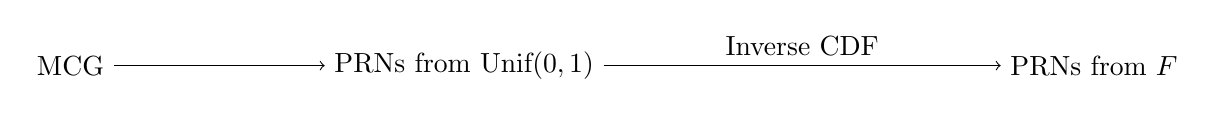
\begin{tikzpicture}
                \node (MCG) at (0, 0) {MCG};
                \node (U) at (5, 0) {PRNs from $\text{Unif}(0, 1)$}; 
                \node (F) at (13, 0) {PRNs from $F$}; 

                \draw[->] (MCG) -- (U); 
                \draw[->] (U) -- (F) node[midway, above]{Inverse CDF};
            \end{tikzpicture}
        \end{center}

    \subsection{Monte Carlo Integration}
        Using the LLN, the LIL, and the PRNG, we can approximate the integral of a function $f: \R^d \to \R$:
        \begin{enumerate}
            \item The PRNG gives us $X_1, X_2, \dots, X_n \iid p$
            \item Using the LLN, we calculate $\hat v_n = \frac{1}{n} \sum_{i=1}^n f(X_i) \approx \E f(X_1) = v$ (where $v$ can be a very complicated integral)
            \item The LIL quantifies this error
        \end{enumerate}
        
    \subsection{Importance Sampling}
        \emph{Goal:} compute 
        \[v = \underbrace{\int \dots \int}_{d integrals} G(x_1, \dots,\; x_d) \; dx_1, \dots dx_d = \int_{\R^d} H(\vec x)\; dx\] 

        We choose a d-dim PDF $f(\vec x)$ such that $f(\vec x)$ is ``similar to'' $\frac{H(\vec x)}{\int H(\vec x)\; d\vec x}$. This allows us to write 
        \[v = \int H(\vec x) \;d \vec x = \int \frac{H(\vec x)}{f(\vec x)} \cdot f(\vec x)\; d\vec x = \E[\frac{H(\vec X)}{f(\vec X)}]\]
        (where the final $\vec X \sim f$)

        When 
        \[f(\vec x) = \prod_{i=1}^d x_i\]
        we can generate random numbers such that 
            ...
        so 
        \[\hat v_n = \frac{1}{n}\sum_{i=1}^n \frac{H(\vec X_i)}{f(\vec X_i)} \approx \int H(\vec x)\; d\vec x\] 

        This method is preferred when $d$ is large. 

    \subsection{Markov Chain Monte Carlo}
        \emph{Motivation:} In general, it is infeasible to generate random vectors from a high dimensional distribution 

        \textbf{Ergodic Theorem:} Let $\{X_n\}_{n=0}^\infty$ be a homogeneous Markov Chain with state space $\mfX = \{x_1, x_2, \dots,\; x_S\}$. If the MC is
        \begin{enumerate}
            \item irreducible
            \item aperiodic
            \item has a unique stationary distribution $\pi:\mfX \to [0, 1]$
        \end{enumerate}
        then
        \begin{enumerate}
            \item \[\lim_{n\to \infty} \P(X_n = y \; | \; X_0 = x) = \pi(y) \\quad x, y \in \mfX\] 
            \item \[\lim_{n\to\infty} \P(X_n = y) = \pi(y)\]
            \item \[\lim_{n\to \infty} \frac{1}{n} \sum_{i=1}^n f(X_i) = \sum_{x \in \mfX} \pi(x) \cdot f(x) = \E[f(\xi)]\]
            ($\xi \sim \pi$)
        \end{enumerate}

        \emph{Conclusion:} If $\{X_n\}_{n=0}^\infty$ is such a MC, 
        \begin{itemize}
            \item When $n$ is large, $X_n \dot \sim \pi$ 
            \item \[\hat v_n = \frac{1}{n} \sum_{i=1}^n f(X_i) \approx \sum_{x \in \mfX} \pi(x)\cdot f(x)\]
        \end{itemize}

        
        That is, given an HMC $\{X_n\}_{n=0}^\infty$, we can calculate $p(x, y) = \P(X_{n+1} = y \; | \; X_n = x)$ to find \emph{the} solution to 
        \[\pi(x) = \sum_{y\in \mfX} \pi(y) \cdot p(y, x) \quad \forall x\in \mfX\]

        To go the other direction (to find an HMC given $\pi$) is harder but can be accomplished with 
        \begin{itemize}
            \item The Metropolis Hastings Algorithm
            \item Gibbs Sampling
        \end{itemize}

    \subsection{Gibbs Sampling}
        Gibbs sampling works only if the model in question is a Gibbs Random Field. 

        \textbf{Gibbs Random Field:} Let $\mfX = \{x_1, x_2, \dots,\; x_S\}$ be a finite set of states. A probability distribution $\pi$ on $\mfX$ is a \emph{Gibbs Random Field} on a graph $G = (V, E)$ with $V ={1, 2, \dots, \; d}$ if 
        \[\pi(x_1, \dots,\; x_d) = \frac{1}{Z} \pi_{c \in C(G)} \phi_c(x_c)\]

        If 
        \[\pi_{i \; | \; -i}(x_i \; | \; x_1, \dots, x_{i-1}, x_{i+1}, \dots,\; x_d)\] 
        depends only on $x_j$ with $j \in N(i) \cup \{i\}$, then $\pi$ is called a Markov Random Field (MRF) WRT G. 

        \textbf{Theorem (Hammersley-Clifford):} Iff $\pi$ is a GRF with respect to a graph, it is a MRF
\end{document}   


